

\documentclass[8pt, usepdftitle=false]{beamer}
% \imput{../common/beamerthemesimple}
\usetheme{simple}


  \usepackage{xcolor}
  \definecolor{olive}{rgb}{0.3, 0.4, .1}
  \setbeamercolor{itemize/enumerate body}{fg=black}
  \setbeamercolor{title}{fg = green!30!black}
  \setbeamercolor{frametitle}{fg = gray!70!black, bg = white}


% \usepackage{lmodern}
\usepackage[scale = 2]{ccicons}
\usepackage[export]{adjustbox}
\usepackage{amsmath, amsthm, amssymb}
\usepackage{amsfonts}
\usepackage{mathtools}

\usepackage[justification=raggedright,width=\linewidth]{caption}
\usepackage{tikz} 


\usepackage{setspace}

\setbeamertemplate{title page}[default][right,colsep=-4bp,rounded=true,shadow=\beamer@themerounded@shadow]

\setbeamertemplate{caption}[numbered]


%% Options

\setbeamercolor{alerted text}{fg=blue}
\setbeamertemplate{alerted text begin}{\itshape}
\setbeamertemplate{alerted text end}{}

\newenvironment<>{varblock}[2][\textwidth]{%
    \setlength{\textwidth}{#1}
    \begin{actionenv}#3%
        \def\insertblocktitle{\underline{#2}}%
        \par%
        \usebeamertemplate{block begin}}
        {\par%
        \usebeamertemplate{block end}%
    \end{actionenv}}

\setbeamertemplate{blocks}[rounded][shadow=true]
\setbeamercolor{block title}{fg=black,bg=gray!20!white}
\setbeamercolor{block body}{fg=black,bg=gray!10!white}




%% Theorem

% \newtheorem{theorem}{Theorem}

%% Bangla tex


\usepackage{polyglossia}
\setotherlanguage[numerals=Devanagari]{bengali}
\setmainlanguage{english}
\newfontfamily\bengalifont[Script=Bengali]{Akaash}


%% tikx

\usepackage{tikz}
\usetikzlibrary{calc,trees,positioning,arrows,fit,shapes,calc}





\newcommand\blfootnote[1]{%
  \begingroup
  \renewcommand\thefootnote{}\footnote{#1}%
  \addtocounter{footnote}{-1}%
  \endgroup
}



\newcommand\Permute[2][^n]{\prescript{#1\mkern-2.5mu}{}P_{#2}}
\newcommand\Combine[2][^n]{\prescript{#1\mkern-0.5mu}{}C_{#2}}


\renewcommand*{\thefootnote}{\fnsymbol{footnote}}


\usepackage{flexisym}
\usepackage{breqn}

\usepackage[T1]{fontenc}

% \usepackage{mathpazo}
% \renewcommand{\rmdefault}{put}

% \usepackage{fourier} 
% Only use the math font of mathpazo
% \let\temp\rmdefault
% \usepackage{mathpazo}
% \let\rmdefault\temp
% \renewcommand{\rmdefault}{put}


% \usepackage[hyphens]{url}


  % \usefonttheme{professionalfonts} % using non standard fonts for beamer
  % \usefonttheme{serif} % default family is serif

  % \usepackage{gentium}
  \usepackage{multicol}
  \usepackage{mathpazo}



% \renewcommand{\familydefault}{\sfdefault}  


  % color brackets
  \makeatletter
  \newcount\bracketnum
  \newcommand\makecolorlist[1]{%
      \bracketnum0\relax
      \makecolorlist@#1,.%
      \bracketnum0\relax
  }
  \def\makecolorlist@#1,{%
      \advance\bracketnum1\relax
      \expandafter\def\csname bracketcolor\the\bracketnum\endcsname{\color{#1}}%
      \@ifnextchar.{\@gobble}{\makecolorlist@}%
  }
  \let\oldleft\left
  \let\oldright\right
  \def\left#1{%
      \global\advance\bracketnum1\relax 
      \colorlet{temp}{.}%
      \csname bracketcolor\the\bracketnum\endcsname
      \oldleft#1%
      \color{temp}%
  }
  \def\right#1{%
      \colorlet{temp}{.}%
      \csname bracketcolor\the\bracketnum\endcsname
      \oldright#1%
      \global\advance\bracketnum-1\relax
      \color{temp}%
  }
  \makeatother


  \makecolorlist{black,blue,red}






\setbeamertemplate{section in toc}{%
  {\color{firstcolor}\inserttocsectionnumber.}~\inserttocsection}
\setbeamercolor{subsection in toc}{bg=white,fg=black}
\setbeamertemplate{subsection in toc}{%
  \hspace{1.2em}{\color{firstcolor}\rule[0.3ex]{3pt}{3pt}}~\inserttocsubsection\par}


\setbeamerfont{section in toc}{size=\fontsize{6}{8}\selectfont}
\setbeamerfont{subsection in toc}{size=\fontsize{6}{8}\selectfont}
\setbeamerfont{subsection in toc shaded}{size=\fontsize{6}{8}\selectfont}


\makeatletter
\patchcmd{\beamer@sectionintoc}{\vskip1.5em}{\vskip0.5em}{}{}
\makeatother






  \usepackage{twemojis}
  \usepackage{fontspec}
  \usepackage{tikzsymbols}
  \newfontfamily\DejaSans{DejaVu Sans}

% for R
\usepackage[fixed]{fontawesome5}


\setbeamercolor{emph}{fg=red}
\renewcommand<>{\emph}[1]{%
  {\color{purple}\only#2{\rm\itshape}#1}%
}

\setbeamertemplate{frametitle continuation}{}


\usepackage[round,  maxcitenames=10, mincitenames=11]{natbib}
\setlength{\bibhang}{0pt}
\renewcommand{\bibsection}{}
\usepackage{fancybox}


\setbeamertemplate{section page}
{
    \begingroup
    \begin{beamercolorbox}[sep=12pt,center]{section title}
        \usebeamerfont{section title}\insertsection\par
    \end{beamercolorbox}
    \endgroup
}

\setbeamertemplate{subsection page}
{
    \begingroup
    \begin{beamercolorbox}[sep=12pt,center]{section title}
        \usebeamerfont{section title}\insertsection\par
    \end{beamercolorbox}
    \vspace*{-1pt}
    \begin{beamercolorbox}[sep=8pt,center]{subsection title}
        \usebeamerfont{subsection title}\insertsubsection\par
    \end{beamercolorbox}
    \endgroup
}



\newcommand\Var[1]{\mathbb{V}\mathrm{ar}{#1}}



\renewcommand{\emph}[1]{%
{\rm\itshape{\color{purple}#1}}%
}

\renewcommand{\alert}[1]{%
{\rm\itshape{\color{blue}#1}}%
}

\newcounter{mytheorem}
\renewcommand{\themytheorem}{3.\arabic{mytheorem}}
\newcommand{\Thm}[1]{\refstepcounter{mytheorem}\textbf{#1\color{blue}\themytheorem}:}




%================ Give the title ============================##

\title{\LARGE Ch3 - Probability Theory - 2}

\subtitle{{\fontsize{10}{10}\selectfont\color{gray!50!balck} 
(Random Variables and Probability Distributions)} \\
\vspace*{.2cm} Statistics For Business and Economics - I}


\author{Shaikh Tanvir Hossain\vspace*{-.4cm}}
\institute{ East West University, Dhaka\\ Last Updated \today}
\date{\vspace{-5pt}}
% \titlegraphic{\includegraphics[width=300,height=.5\textheight]{Images/EWU.png}}

% \setbeamertemplate{background}{\tikz[overlay,remember picture]\node[opacity=0.90]at (current page){\includegraphics[width=.5\textwidth,left]{EWU.png}};}



\usepackage{hyperref}
\hypersetup{
      pdftitle={Ch3 - Probability Theory - 2},
        pdfauthor={Shaikh Tanvir Hossain},
          pdfborder={0 0 0},
       colorlinks,
      citecolor=blue,
      linkcolor=gray!50!black,
    breaklinks=true}





\begin{document}

% input the outline 

\begin{frame}[plain,noframenumbering] 
    \maketitle
\end{frame}
\setbeamertemplate{background}{}
\setlength{\abovedisplayskip}{-2pt}
\setlength{\belowdisplayskip}{4pt}
\setlength{\abovedisplayshortskip}{-3pt}
\setlength{\belowdisplayshortskip}{4pt}


\AtBeginSection[]
{
    \begin{frame}[plain, allowframebreaks]
\setstretch{.1}

        \setlength{\parskip}{1ex}
            \tableofcontents[sections={1-7}, 
            currentsubsection, 
            sectionstyle=show/hide, 
            sectionstyle=show/shaded, 
            ]
    \end{frame}
}


% Hide progress bar and footline on titlepage
\begin{frame}{Outline}
 \vspace*{.2cm}

\begin{center}
\begin{minipage}{10cm}
  \begin{alertblock}{Outline}
  \setstretch{.1}
   \setlength{\parskip}{1ex}
  \tableofcontents[sections={1-10}]
  %   \framebreak
  % \tableofcontents[sections={2}]
\end{alertblock}
\end{minipage}
\end{center}


\end{frame}



\begin{frame}[allowframebreaks]{}

\begin{itemize}
\item In this chapter we start with the second part of the probability theory where we will start talking about \emph{random variables} and \emph{probability distributions}. Undoubtedly these two concepts are really the core part of Probability Theory and Statistics. In this chapter we will cover univariate random variables and some univariate probability distributions. These are theoretical distributions which are useful to \alert{model} real life scenarios for one variable only. The next chapter will be about multivariate random variables and joint probability distributions (along with conditional distributions) which is more like an extension of these ideas to multivariate setting.

\item So let's start...\faWalking \faWalking \faWalking.

\end{itemize}

\end{frame}



%---------------------------------------------------------------------------------
\section{Random Variables}
\frame{\sectionpage}

\subsection{Definitions, Discrete and Continuous}
\frame{\subsectionpage}



\begin{frame}[allowframebreaks]{Random Variables}{Definitions, Discrete and Continuous}

\begin{itemize}

\item What is a random variable? Sometimes we are not interested in the experimental outcome directly, rather we are interested in some \emph{function of the experimental outcome}. Here is an example. 

\item \Thm{Example } (Three coin toss experiment) Suppose we are doing the experiment of tossing $3$ independent coins. Then we know the experimental outcomes are (recall $\Omega$ is the sample space)

\begin{align*}
\Omega = \{{(H, H, H)}, {(H,H,T)}, {(H,T,H)}, {(T,H,H)}, \\
{(T,T,H)}, {(T,H,T)}, {(H,T,T)}, {(T,T,T)} \}
\end{align*}  

\item Now suppose we are NOT interested in these outcomes, rather we are interested in the \emph{``total number of heads''} for each experimental outcome. For example, for the first outcome ${(H, H, H)}$, the total number of heads is $3$, for the second outcome ${(H,H,T)}$, the total number of heads is $2$, etc. 

\item We can represent this as function $X : \Omega \to \mathbb{R}$, where the domain is $\Omega$ and co-domain is $\mathbb{R}$.

 \item Here we can think $X(\omega)$ is a function where $\omega$ is the input that is coming from the sample space $\Omega$, and the output will be total number of heads, which is going to be a number in $\mathbb{R}$.


\begin{figure}
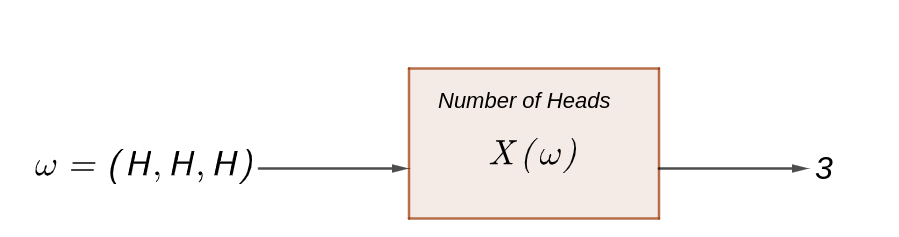
\includegraphics[scale = .3]{Images/Function_1.png}
\end{figure}

\framebreak

\item In this way we can think about all outcomes of this experiments and the value of the function $X(\omega)$


\begin{align*}
\begin{array}{ccccc}
\hline \omega &  {(H,H,H)} &  {(H,H,T)} &  {(H,T,H)} &  {(T,H,H)} \\
\hline X(\omega) & 3 & 2 & 2 & 2 \\
\hline \\
\hline \omega &    {(T,T,H)} &  {(T,H,T)} &  {(H,T,T)} &  {(T,T,T)} \\
\hline X(\omega)  & 1 & 1 & 1 & 0 \\
\hline
\end{array}
\end{align*}

\item \alert{Here $X$ is a random variable, and it's values are $0, 1, 2, 3$}. 

\item So a random variable is a function which takes input from the sample space $\Omega$ and gives us a number in the real line $\mathbb{R}$.


\framebreak

\item Notice in the last example, the random variable \emph{cannot take any values in $\mathbb{R}$}. It can only take $4$ values, $0, 1, 2, 3$.  So we can write the \alert{range of the function} as $\mathcal{X} = \{0, 1, 2, 3\}$.

\item Depending upon whether the range $\mathcal{X}$ is a \emph{countable set or uncountable set}, we can classify the random variables into two types. 

\medskip
\begin{itemize}
	\item \alert{Discrete Random Variable}: When the range of the random variable $\mathcal{X}$ is a countable set, for example $\mathcal{X} = \{0, 1, 2, 3\}$, we call it discrete random variable. Important $\mathcal{X} = \{0, 1, 2, 3, \ldots\}$, is also a countable set, we call it infinitely countable set.
	
	\medskip
	\item \alert{Continuous Random Variable}:  When the range of the random variable $\mathcal{X}$ is an uncountable or infinite set, we call it a continuous random variable, for example $\mathcal{X} = [0, 1]$ or even $\mathcal{X} = \mathbb{R}$
\end{itemize}
\medskip

\item Now we can write the formal definition of a random variable,

\begin{varblock}{\Thm{Definition } (Random Variables, discrete and continuous)}

A Random Variable $X(\omega)$ is a function, we write $X:\Omega \to \mathbb{R}$. If the range $\mathcal{X}$ of this function a countable set we call the random variable \alert{a discrete random variable}, and if the range $\mathcal{X}$ is an uncountable set we call it \alert{a continuous random variable}. Usually the random variables are denoted with uppercase letters $X$, $Y$, $Z$ or $W$ and often the input $\omega$ is  suppressed. 
\end{varblock}



\item Again, recall, $X: \Omega \to \mathbb{R}$, means $X$ is a function, $\Omega$ is the \emph{domain} of the function, $\mathbb{R}$ is the \emph{codomain}. 

\item Also as we mentioned before, we will denote $\mathcal{X}$ as the range of the function. 


\framebreak

\item In the last example, can you think about other random variables defined on the same sample space? ... (Ans: Yes we can, for example think about total number of tails, whether we have at least two heads, or whether we have at least one tail, etc.)


\item In principle it is \emph{possible to define many random variables} on the same sample space.

\item As we wrote in the definition, we will use the uppercase letters such that $X$, $Y$, $Z$, etc., to denote the random variables. The lower case letters $x$, $y$, $z$, etc., will be used to denote the values of the random variables. For example it can be $X(\omega) = x$, this means if the experimental outcome is $\omega$, the random variable $X$ will take value $x$.

\item You might be wondering why we call this \emph{``random''} variable? Any guess? This is because before performing the experiment, the \alert{input of the function is random}. So the \alert{output of the function is also random}. 


\item Note that there is a difference between a mathematical function $f(x)$ (which is non-random) and a random variable $X(\omega)$ which is also a function? 

\item For a random variable the input is a random object, but when we are thinking function generally in mathematics we think about a fixed / non-random input (there is no experiment going on in the background!)


\framebreak


\begin{figure}
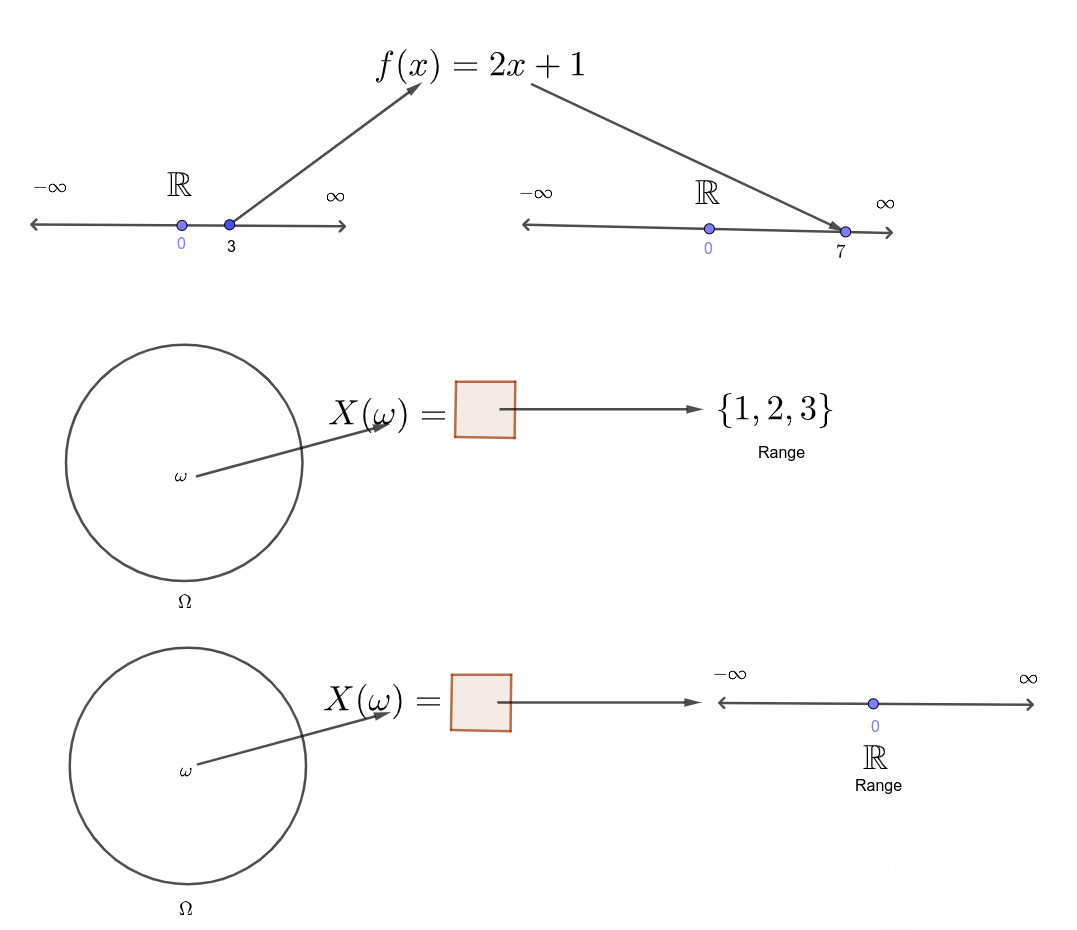
\includegraphics[scale = .2]{Images/RVs_OFs.png}
\caption{From the top, the first one is a mathematical function where the input is not random and the output is also not random (we often call this deterministic function). Here $f: \mathbb{R} \to \mathbb{R}$, and also the range is $\mathbb{R}$. The second one is a discrete random variable where the range is $\mathcal{X} = \{1, 2, 3 \}$. And the third one is a continuous random variable where the range is $\mathcal{X} = \mathbb{R}$. Note that for the random variables there is a blank box, this means before performing the experiment we don't know the output.}
\end{figure}


\item Let's see an example of a continuous random variable (example taken from \cite{degroot_probability_2012})


\item Suppose a contractor is building an office complex and needs to plan for water and electricity demand. After consulting with prospective tenants and examining historical data, the contractor decides that the demand for electricity will range somewhere between 1 million and 150 million kilowatt-hours per day and water demand will be between 4 and 200 (in thousands of gallons per day). All combinations of electrical and water demand are considered possible. In this case we have the following sample space 

\begin{figure}
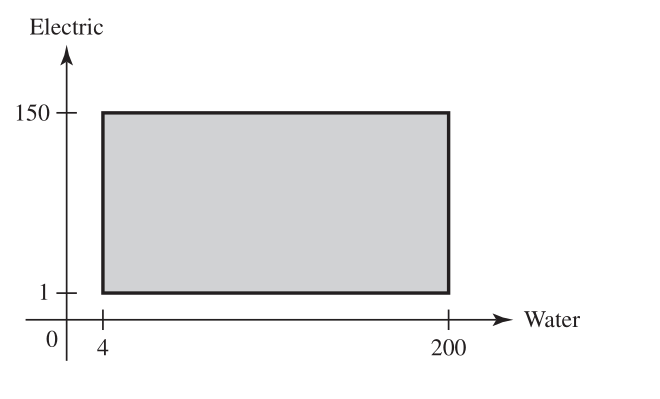
\includegraphics[scale = .25]{Images/CRV_1.png}
\caption{This is the sample space $\Omega$ of the experiment, notice the sample space is an infinite set}
\end{figure}

\item The shaded region shows the sample space for the experiment, consisting of learning the actual water and electricity demands for the office complex. 

\item Here we can express the sample space as a Cartesian Product $[4, 200] \times [1, 150]$ or set of all ordered pairs $(x, y)$ where $4 \leq x \leq 200$ and $1 \leq y \leq 150$,


\begin{align*}
\Omega &=  [4, 200] \times [1, 150] \\
&=\{(x, y): 4 \leq x \leq 200,1 \leq y \leq 150\}
\end{align*}

\item where $x$ stands for water demand in thousands of gallons per day and $y$ stands for the electric demand in millions of kilowatt-hours per day.

\item We can also think about different events, which is going to be a subset of the sample space $\Omega$.

\begin{align*}
A &= \{(x, y) ; x \geq 100, 1 \leq y \leq 150\} \text{ or maybe }\\
B &= \{(x, y): 4 \leq x \leq 200, y \geq 115\}
\end{align*}

\item $A$ means water demand is \emph{at least $100$}, 

\item $B$ means electricity demand \emph{at least $115$}. 

\item What if we write $C = \{(x, y): x \geq 100, y \leq 35\}$, can you interpret this?

\item This sample space has infinitely many points, and note carefully that the sample space is uncountable. 

\framebreak

\item Now we can think about different random variables defined here.


\item For example, One random variable that is of interest is the demand for water. This can be expressed as $X(\omega) = x$ when $\omega=(x, y)$.  The possible values of $X$ are the numbers in the interval $[4,200]$, so in this case the range is $\mathcal{X} = [4, 200]$. So this is a continuous random variable.

\item Another random variable is $Y$ where it's value will be the electricity demand, which can be expressed as $Y(\omega)=y$ when $\omega=(x, y)$. The possible values of $Y$ are the numbers in the interval $[1,150]$. Again this is also an example of continuous random variable.

\framebreak

\item Another possible random variable could be $Z$, where $Z$ is an \alert{indicator of} whether or not at least one demand is high. Let $A$ and $B$ be the two events described before, that is, $A$ is the event such that water demand is at least 100 , and $B$ is the event such that electricity demand is at least 115 . Define

$$
Z(\omega)= \begin{cases}1 & \text { if } \omega \in A \cup B, \\ 0 & \text { if } \omega \notin A \cup B,\end{cases}
$$

\item The possible values of $Z$ are the numbers 0 and 1 . The event $A \cup B$ is shown in the following figure, which represents the area of the sample space where at least one demand is high.


\begin{figure}
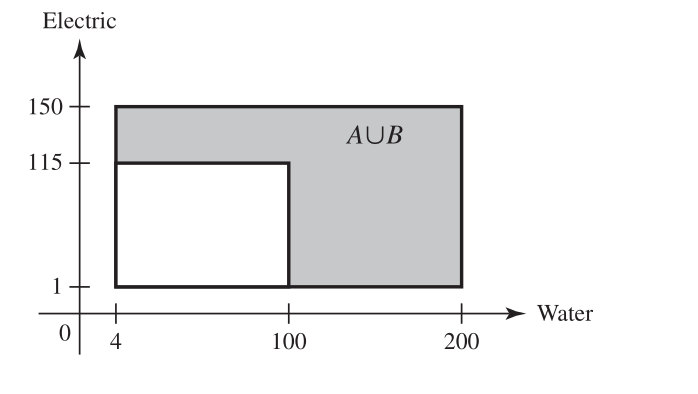
\includegraphics[scale = .25]{Images/CRV_2.png}
\caption{$A\cup B$ is the shaded area where water demand is at least $100$ or electricity demand is at least $115$}
\end{figure}


\item Let's see some real life examples of random variables. It's important that in many cases the random variable and the values are clear but the sample space is probably not clear. So when we start thinking about random variables, we don't actually think about the actual sample space, rather we think about the random variable and the values it can take. 


\item Following are some examples of discrete random variable  (some examples are taken from \citet*{anderson_statistics_2020}).



\small{
\begin{table}[H]
\begin{tabular}{l|l|l} 
\emph{Random Experiment} & \emph{RV - $X$} & \emph{Possible Values, $x$ } \\ \hline
Toss a coin & 1 - head, 0 - tail & $1, 0$  \\
Roll a die & \# dots in upper face & $1,2,3,4,5,6$ \\
Contact a single customers & 1 - receives, 0 - ignores & $1,0$ \\
Contact $5$ customers & \# customers who receives & $0,1,2,4,5$ \\
Operate a hospital for a day & \# patients who arrive & $0,1,2,3, \ldots$ \\
Offer a customer the choice of  products & product chosen by customer & 
0 - None, 1 - A, 2 - B \\
Randomly pick $10$ EWU students & their occupation status & 1 - job, 0 - no job
\end{tabular} 
\caption{Examples of Discrete Random Variables}		
\end{table}
}

\small{
\raggedright
\begin{table}[H]
\begin{tabular}{l|l|l} 
\emph{Random Experiment} & \emph{RV - $X$} & \emph{Possible Values, $x$ } \\ \hline
Customer visits a web page & time customer spends (in min) & $[0, \infty)$ \\
Taking a bus to Uni & time you have to wait (in min) & $[0, \infty)$ \\
Randomly pick $10$ EWU students & their heights (in cm) & $[120, 210]$ \\
A flight from Dhaka to Chittagong & time need to travel (in min) & $[60, 90]$ \\

\end{tabular}
\caption{Examples of Continuous Random Variables}		
\end{table}
}


\end{itemize}
\end{frame}




\subsection{Calculating Probabilities and Distributions}
\frame{\subsectionpage}


\begin{frame}[allowframebreaks]{Random Variables}{Calculating Probabilities and Distributions}

\begin{itemize}


\item There is a very important point of thinking about random variables, that is


\vspace*{.2cm}
\emph{Once we start thinking about random variables, now we have a \alert{new sample space $\mathbb{R}$}, then we can think about \alert{different events in the new sample space $\mathbb{R}$}, and forget about the original sample space $\Omega$}
\vspace*{.2cm}


\item Since now we have a new sample space $\mathbb{R}$, we can think about different events in $\mathbb{R}$ (which are subsets of $\mathbb{R}$) and then maybe we can calculate probability in these events, for example 

\begin{align*}
	&\mathbb{P}([1, 1.5)) \\
	&\mathbb{P}([4, 10000)) \\
	&\mathbb{P}(  [1, 2)) \\
\end{align*}


\item Note that since $\mathbb{R}$ is sample space in this case, we will always have $\mathbb{P}(\mathbb{R}) = 1$. 


\item Also note if $X$ is a random variable, for the probabilities we wrote above, we can write them as,


\begin{align*}
	&\mathbb{P}(X \in [1, 1.5)) \text{ or we write } \mathbb{P}( 1 \leq X <  1.5)\\
	&\mathbb{P}(X \in [4, 10000)) \text{ or we write } \mathbb{P}( 4 \leq X <  10000)\\
	&\mathbb{P}(X \in [1, 2)) \text{ or we write } \mathbb{P}( 1 \leq X <  2)\\
\end{align*}


\framebreak

\item \alert{CAVEAT \faMugHot :} It turns out that it is not easy to calculate probabilities in $\mathbb{R}$, and there might be some issues, there are some bad sets / intervals where we cannot calculate probabilities with a consistent way. To explain it fully we need to talk about measurability issues, which is beyond the scope of this course, so we will simply assume that it is possible to calculate probabilities in the interval of $\mathbb{R}$, and you can ignore this comment if you want!


\framebreak

\item Now how do we calculate probabilities of these events or intervals in $\mathbb{R}$?


\item Let's do one example, say we want to calculate the probability $\mathbb{P}([1, 1.5))$ for the random variable defined in Example 3.1. 


\item It turns out for this random variable in Example 3.1, if we know following probabilities,

\begin{itemize}
	\item $\mathbb{P}(\{0\}) = \mathbb{P}(X = 0)$ or probability that the random variable will take value $0$ and 
	\item $\mathbb{P}(\{1\}) = \mathbb{P}(X = 1)$ or probability that the random variable will take value $1$ and
	\item $\mathbb{P}(\{2\}) = \mathbb{P}(X = 2)$ or probability that the random variable will take value $2$ and 
	\item $\mathbb{P}(\{3\}) = \mathbb{P}(X = 3)$ or probability that the random variable will take value $3$,
\end{itemize}


\item then we can calculate probability of any interval in $\mathbb{R}$ for this random variable. 

\item Here is how we can do this, we can find the event associated with each value and then calculate the probability of that event using classical definition, for example 

\begin{align*}
	 X &= 0 \text{ is associated with the event } \{ (T, T, T)\} \\
 	 X &= 1 \text{ is associated with the event } \{ (H,T,T), (T,H,T), (T,T,H)\} \\
	 X &= 2 \text{ is associated with the event } \{ (H,H,T), (H,T,H), (T,H,H)\} \\
	 X &= 3 \text{ is associated with the event } \{ (H,H,H)\}\\
\end{align*}


% \item This is because, 


% \begin{align*}
% \begin{array}{ccccc}
% \hline \omega &  {(H,H,H)} &  {(H,H,T)} &  {(H,T,H)} &  {(T,H,H)} \\
% \hline X(\omega) & 3 & 2 & 2 & 2 \\
% \hline \\
% \hline \omega &    {(T,T,H)} &  {(T,H,T)} &  {(H,T,T)} &  {(T,T,T)} \\
% \hline X(\omega)  & 1 & 1 & 1 & 0 \\
% \hline
% \end{array}
% \end{align*}

 
%  \item Now we can calculate $\mathbb{P}(\{ (H,T,T), (T,H,T), (T,T,H)\})$, and then that will be $\mathbb{P}(X =1)$.


\item Now applying the classical definition with equally likely assumption we get,



\begin{align*}
	\mathbb{P}\left(\{ (H,T,T), (T,H,T), (T,T,H)\}\right)=\frac{3}{8}
\end{align*} 



\item So this means, now we know 

\begin{align*}
	\mathbb{P}(X =1)=\mathbb{P}\left(\{ (H,T,T), (T,H,T), (T,T,H)\}\right)=\frac{3}{8}
\end{align*}



\item With the same idea applied we can calculate other probabilities, 

\begin{align*}
\begin{array}{ccccc}
\hline x & 0 & 1 & 2 & 3 \\
\hline \mathbb{P}(X=x) & \frac{1}{8} & \frac{3}{8} & \frac{3}{8} & \frac{1}{8} \\
\hline
\end{array}
\end{align*}

\item Here $ \mathbb{P}(X=x)$ means, probability of $X$ taking values $x$, where $x$ can be $0$, $1$, $2$ and $3$. Please try to calculate the other values.



\item So with this approach we can actually get the Probabilities of a random variable $X$ taking different values.

\item And now we can also calculate the following probabilities 

\medskip
\begin{itemize}
	\item  $\mathbb{P}( X \in [1, 1.5)) $  or 
	\item $\mathbb{P}( X \in [4, 10000)) $ or 
	\item $\mathbb{P}( X \in [1, 2)) $ or 
	\item any other interval in $\mathbb{R}$
\end{itemize}
\medskip



\item How? Just use the probabilities where $X$ actually takes its values, for example,

\begin{align*}
\mathbb{P}( X \in [1, 1.5)) = \mathbb{P}(X = 1) =  \frac{3}{8}
\end{align*}

\item Why $\frac{3}{8}$? The reason is in this interval $X$ does not take values other than $1$, so all the other points in this interval have probability $0$.


\item Can you do the other calculation in page 16? Yes, but we can do more

\item In fact with these 4 probabilities, for this random variable we can calculate the probability of \alert{any interval in $\mathbb{R}$}.

\item Here for a random variable $X$, the probability distribution means how the probabilities are distributed on the real line $\mathbb{R}$.

\begin{varblock}{Distribution of a random variable}
	Let $X$ be a random variable. The distribution of $X$ is the collection of all probabilities of the form $\mathbb{P}(X \in C)$ for all sets $C$ of real numbers such that $\{X \in C\}$ is an event.
\end{varblock}



\framebreak


\item Do you think we always have to find probabilities by going back to original sample space? The answer is NO.

\item There are actually two nice functions on the real line $\mathbb{R}$, which helps to calculate probabilities when the random $X$ takes values in different kinds of intervals.

\item For discrete random variable this function is known as \alert{probability mass function} or in short \alert{PMF} and for continuous random variable this function is known as \alert{probability density function} or in short \alert{PDF}.

\item Next we will see the discussion for Discrete Probability Distributions and Continuous Probability Distributions and we will talk about PMF and PDF and their use in detail.






\end{itemize}
\end{frame}


% \begin{frame}{Random Variables}


% \begin{itemize}

% \item So we have seen what is a random variable, mathematically it's a function defined on the sample space.

% \item Intuitively it somehow transforms the outcomes of the experiments and give us a number.

% \item \cite{anderson_statistics_2020} defines the random variable as \emph{as a numerical description of the outcome of an experiment}. This definition gives us a nice intuitive idea about random variables, but mathematically not precise.

% \item So we defined the random variable using function\footnote[frame]{Similar definitions can be found in \cite{casella_statistical_2002}, \cite{degroot_probability_2012}, \cite{blitzstein_introduction_2015}, \cite{bertsekas2008introduction} and in many other textbooks}. If you have understood functions, you should automatically understand what is a random variable.


% \item You should always think about following picture if you think about random variables.



% \end{itemize}



% \end{frame}



% \begin{frame}{Random Variables}




% \end{frame}

% \begin{frame}{Random Variables}

% \begin{itemize}
% \item The random variable that we have seen in page 6 and page 7 might look a bit abstract. But there are many real-life examples of random variables, in particular you can look at table $5.1$ and $5.2$ in \cite{anderson_statistics_2020}. 



% \end{itemize}

% \end{frame}





% \section{Distribution of a Random Variable (Basic idea)}
% \frame{\sectionpage}


% \begin{frame}[allowframebreaks]{Distributions of Random Variables}{General Idea}

% \begin{itemize}

% \item Once we understand what is a random variable, the next topic for us is to understand the \emph{probability distribution} or we say \emph{distribution of a random variable}. 


% \item The word \alert{distribution} here roughly mean \emph{how probabilities are distributed over the values of the random variable}.


% % \item First note, the moment we define a random variable $X$, we have \alert{automatically created a new sample space}. What is this new sample space?

% % \item This is the range of $X$, or $\mathcal{X}$. 

% \item For example, consider the range of the random variable $X$ in the first example,

% \begin{align*}
% \mathcal{X} = \{0, 1, 2, 3\}
% \end{align*}  


% \item We want to know following probabilities,


% \begin{itemize}
% 	\item $\mathbb{P}(X = 0)$ or probability that the random variable will take value $0$. 
% 	\item $\mathbb{P}(X = 1)$ or probability that the random variable will take value $1$. 
% 	\item $\mathbb{P}(X = 2)$ or probability that the random variable will take value $2$. 
% 	\item $\mathbb{P}(X = 3)$ or probability that the random variable will take value $3$.
% \end{itemize}


% \item How can we calculate these probabilities? One idea we can find the event associated with each value and then calculate the probability of that event.

% \framebreak

% \item For example 

% \begin{align*}
% 	 X = 1 \text{ is associated with the event } \{ (H,T,T), (T,H,T), (T,T,H)\}
% \end{align*}


% \item This is because this is the set of outcomes where we have $X = 1$, recall the table,


% \begin{align*}
% \begin{array}{ccccc}
% \hline \omega &  {(H,H,H)} &  {(H,H,T)} &  {(H,T,H)} &  {(T,H,H)} \\
% \hline X(\omega) & 3 & 2 & 2 & 2 \\
% \hline \\
% \hline \omega &    {(T,T,H)} &  {(T,H,T)} &  {(H,T,T)} &  {(T,T,T)} \\
% \hline X(\omega)  & 1 & 1 & 1 & 0 \\
% \hline
% \end{array}
% \end{align*}

 
%  \item Now we can calculate $\mathbb{P}(\{ (H,T,T), (T,H,T), (T,T,H)\})$, and then that will be $\mathbb{P}(X =1)$.


% \item Applying the classical definition with equally likely assumption we get,



% \begin{align*}
% 	\mathbb{P}\left(\{ (H,T,T), (T,H,T), (T,T,H)\}\right)=\frac{3}{8}
% \end{align*} 



% \item So this means, now we know 

% \begin{align*}
% 	\mathbb{P}(X =1)=\mathbb{P}\left(\{ (H,T,T), (T,H,T), (T,T,H)\}\right)=\frac{3}{8}
% \end{align*}




% \item With the same idea applied we can calculate other probabilities, 

% \begin{align*}
% \begin{array}{ccccc}
% \hline x & 0 & 1 & 2 & 3 \\
% \hline \mathbb{P}(X=x) & \frac{1}{8} & \frac{3}{8} & \frac{3}{8} & \frac{1}{8} \\
% \hline
% \end{array}
% \end{align*}

% \item Here $ \mathbb{P}(X=x)$ means, probability of $X$ taking values $x$, where $x$ can be $0$, $1$, $2$ and $3$. Please try to calculate the other values.



% \item So with this approach we can actually get the Probabilities of a random variable $X$ taking different values.

% \item And now we can also calculate the following probabilities 

% \medskip
% \begin{itemize}
% 	\item  $\mathbb{P}( X \in [1, 1.5)) $  or 
% 	\item $\mathbb{P}( X \in [4, 10000)) $ or 
% 	\item $\mathbb{P}( X \in [1, 2)) $ or 
% 	\item any other interval in $\mathbb{R}$
% \end{itemize}
% \medskip



% \item How? Just use the probabilities where $X$ actually takes its values, for example,

% \begin{align*}
% \mathbb{P}( X \in [1, 1.5)) = \mathbb{P}(X = 1) =  \frac{3}{8}
% \end{align*}

% \item Why $\frac{3}{8}$? The reason is in this interval $X$ does not take values other than $1$, so all the other points in this interval have probability $0$.


% \item Can you do the other calculation?

% \framebreak

% \item We didn't see the formal definition of the distribution of a random variable, but roughly knowing distribution actually means \emph{we know the complete set of probabilities of all kinds intervals in $\mathbb{R}$} where we can assign probability.

% \item So as we have seen that for discrete random variable \emph{knowing the probability of individual outcomes is enough to calculate the probabilities of different intervals in $\mathbb{R}$}.

% \item What about continuous random variables? This is difficult to think, right?

% \item In principle, it is very difficult to characterize the distribution of a random variable $X$, whether it is discrete or continuous.



% \end{itemize}



% \end{frame}
\section{Prob. Dist: PMF, PDF, CDF, $\mathbb{E}(\cdot)$, $\mathbb{V}\mathrm{ar}(\cdot)$}
\frame{\sectionpage}

\subsection{Idea of PMF}
\frame{\subsectionpage}


\begin{frame}[allowframebreaks]{Probability Distributions}{Idea of PMF}

\begin{itemize}

\item The distribution of a discrete random variable is known as \emph{discrete distribution}. 

\item We already saw that to know the probability distribution of a discrete random variable it is enough to know the \emph{probabilities at all values $x$} that the discrete random variable can take.

\item This means we need to know $\mathbb{P}(X = x)$ at all $x$ in the range of $X$.


\item The idea of \emph{Probability mass function or PMF} is just a function of $x$ which gives us $\mathbb{P}(X = x)$ directly, it's like if you know the PMF of a discrete random variable, you know the distribution of the random variable.

\item Here is the formal definition of PMF,

\begin{varblock}{\Thm{Definition } (Probability Mass Function (PMF))}
If $X$ is a discrete random variable then the probability mass function (in short PMF) of $X$, denoted by $f$, is defined as the function such that \alert{for all $x \in \mathbb{R}$},

$$
f(x)=\mathbb{P}(X=x)
$$

The set $\{x: f(x)>0\}$ is called the \alert{support of (the distribution of) $X$}.
\end{varblock}

\item It's important to note that this function is defined for all real numbers but when it has positive values we call the set of those points \emph{the support of the distribution}.


\item For example here is the PMF for the random variable that we have defined in Example 3.1,



\begin{align}\label{pmf_1}
f(x)= \begin{cases} 1/8 & \text { if } x=0 \\ 
3/8 & \text { if } x=1 \\ 
3/8 & \text { if } x=2 \\ 
1/8 & \text { if } x=3 \\ 
0 & \text { otherwise }\end{cases}
\end{align}



\item So for all possible values other than in the support the function has output $0$. Recall, this is actually a \emph{piecewise function} in math.

\item Suppose if someone gives you this function, then you can calculate the probabilities of different intervals in $\mathbb{R}$.



\item Can we plot this function? Yes we can. Here is the plot. 
\begin{figure}
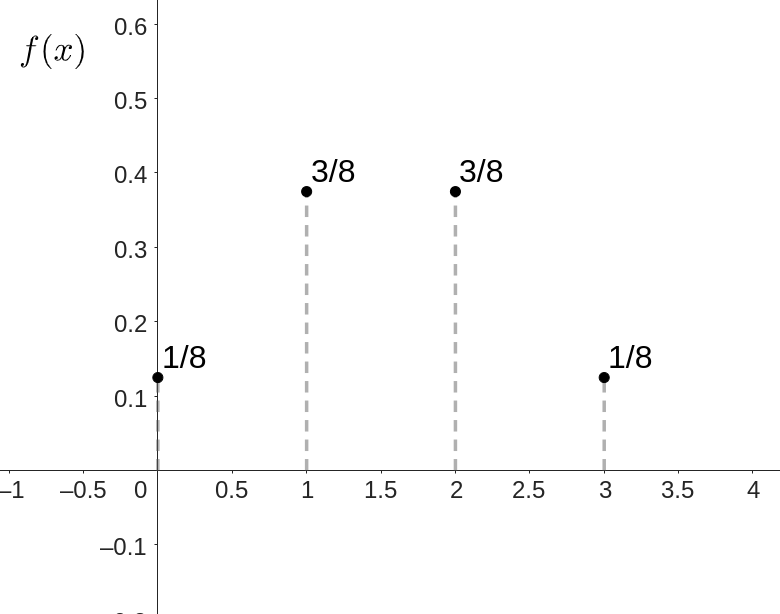
\includegraphics[scale = .3]{Images/pmf_1.png}
\caption{Plot of the PMF in \eqref{pmf_1}} 
\end{figure}

\item The PMF has two important properties, both are easy to understand

\medskip
\begin{varblock}{\Thm{Theorem } (Properties of PMF)}
\begin{itemize}
\item \textbf{The sum of all PMF values is 1}: This means if $x_1, x_2, \ldots$ includes all the possible values of a discrete random variable $X$, then 

\begin{align*}
	\sum_{i=1}^{\infty} f\left(x_i\right)= f(x_1) + f(x_2) + \ldots  = 1
\end{align*}


\item \textbf{The probability of a subset in $\mathbb{R}$ can be calculated as the sum of PMF values in the set}: If  $A$ is any subset of the real line (for example any interval), then we can calculate $\mathbb{P}(X \in A)$ with

$$
\mathbb{P}(X \in A)=\sum_{x_i \in A} f\left(x_i\right)
$$
\end{itemize}

\end{varblock}
\medskip

\item The first one should be obvious, all it says if you sum the PMF functions value, then you should get $1$.  

\item For example, in our 3 coin toss example, we have 

\begin{align*}
	f(0) + f(1) + f(2) + f(3) = 1/8 + 3/8 + 3/8 + 1/8 = 1
\end{align*}


\item The second one says the probability of any interval in $\mathbb{R}$ can be calculated by adding the PMF values in that interval. 

\item We already saw the application of this rule in page 19/38. Recall we calculated 

\begin{align*}
\mathbb{P}( X \in [1, 1.5)) = \mathbb{P}(X = 1) = f(1) =  \frac{3}{8}
\end{align*}


\item The key thing to understand here is knowing PMF is enough to calculate probabilities of different intervals in $\mathbb{R}$.


\framebreak


\item It is important to mention that \cite{anderson_statistics_2020} uses the terminology \emph{probability function} for PMF. But essentially they are same thing. So if you are reading Chapter 5.2 in \cite{anderson_statistics_2020}, then probability function means probability mass function. Because probability mass function or PMF is more common in the literature we will use PMF.

\item Let's see a real life / empirical example of a PMF. Here the idea of the probability mass function is very similar to calculating \emph{relative frequency}, but we need to calculate this using a population. Following example will illustrate this idea.


\framebreak


\item \Thm{Example } (Random Variable and PMF - Empirical Example from \cite{anderson_statistics_2020})


\item Suppose our random variable $X$ is the number of cars sold per day at DiCarlo Motors in Saratoga, New York and we know it can be $0, 1, 2, 3, 4$ or $5$.


\item Now over the past $300$ days, DiCarlo has experienced - 

\begin{itemize}
	\item $54$ days with no (or $0$) automobiles sold, 
	\item $117 $ days with $1$ automobile sold, 
	\item $72$ days with $2$ automobiles sold, 
	\item $42$ days with $3 $ automobiles sold, 
	\item $12$ days with $4$ automobiles sold and 
	\item $3$ days with $5$ automobiles sold.
\end{itemize}


\item If we think this is our population then with this population we can write following probability mass function.


\begin{table}
\centering
\begin{align*}
\begin{array}{c|c}
x & f(x)  \\ \hline
0 & 54/300 = .18 \\
1 & 117/300 = .39 \\
2 & 72/300 = .24 \\
3 & 42/300 = .14 \\
4 & 12/300 = .04 \\
5 & 3/300 = .01
\end{array}
\end{align*}

\end{table}

\item So the PMF is 

\begin{align*}
f(x)= \begin{cases} .18 & \text { if } x=0 \\ 
.39 & \text { if } x=1 \\ 
.24 & \text { if } x=2 \\ 
.14 & \text { if } x=3 \\
.04 & \text { if } x=4 \\
.01 & \text { if } x=5 \\
0 & \text { otherwise }\end{cases}
\end{align*}




\item Note the idea is very similar to calculating relative frequency! This way of thinking is helpful for understanding, but in reality often \emph{we never know the population}, we actually have a sample.

\item From a sample we can never get the probability mass function, what we can get is frequency distribution (this is what we did in chapter 1) 

\item So question is if we don't know the Population what is the solution? Ans - The idea is we will usually \emph{assume the population is distributed according to some theoretical distribution} and then we will model the real life scenarios using some theoretical distribution.

\framebreak

\item There are many theoretical discrete distributions, but we will learn $4$ of them, 

\begin{itemize}
	\item \emph{Discrete Uniform Distribution}, 
	\item \emph{Bernoulli distribution}, 
	\item \emph{Binomial distribution} and 
	\item \emph{Poisson distribution}.
\end{itemize}

\item Now we will start with \alert{Discrete Uniform Distribution}, and will talk about other distributions in coming sections.

\framebreak


\item \alert{Discrete Uniform Distribution} is very simple and you can think this is similar to the idea of equally likely outcomes but this is for the values of the random variable.


\begin{varblock}{\Thm{Definition } (Discrete Uniform Distribution)}
If $X$ can take values $ x_1, x_2, \ldots, x_k$ then we say $X$ follows \alert{Discrete Uniform} distribution with parameter $\{x_1, x_2, \ldots, x_k\}$. The PMF of $X$ is

\begin{align*}
f(x) = \left\{\begin{array}{ll}
\frac{1}{k} & \text { for } x=x_1,x_2, \ldots, x_k \\
0 & \text { otherwise }
\end{array}\right\}
\end{align*}
We write this as $X \sim \mathrm{DUnif}\{x_1, x_2, \ldots, x_k\}$.
\end{varblock}

\item Here parameter determines which specific Uniform Distribution we have and changing the parameter will change the distribution. It will be still a discrete uniform distribution but the distribution will change (see example in the next slide).


\item Note that $X$ can take values in any finite set, the idea of the discrete random variable is the \emph{values will all have equal probabilities}. Let's see a real life example.


\framebreak

\item  Suppose everyday your brother can give you $10$, $20$ or $30$ taka and he might give you any of the three amounts with equal probability. So if we represent the random variable $X$ as the amount of money you will get everyday, then $X$ follows discrete uniform distribution with parameter $\{10, 20, 30\}$, we write $X \sim \mathrm{DUnif}\{10, 20, 30\}$ and the PMF of $X$ is

\begin{align*}
	f(10) &= 1/3, \\
	f(20) &= 1/3 \\
	\text{ and } f(30) &= 1/3.
\end{align*}

\item How does it look like?

\begin{figure}
	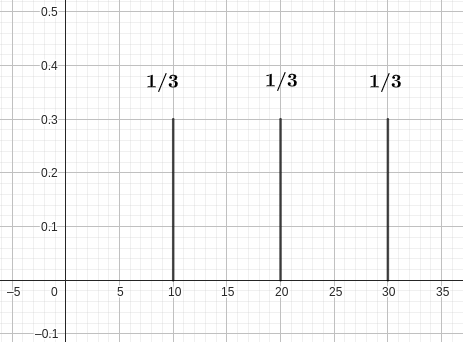
\includegraphics[scale = .4]{Images/DiscreteUniform.png}
\end{figure}

\item Notice here parameter is $\{10, 20, 30\}$, so if we change the parameter, for example, if we change the parameter to $\{10, 20, 30, 40\}$, then the distribution will change.


\end{itemize}

\end{frame}


\subsection{Idea of PDF}
\frame{\subsectionpage}


\begin{frame}[allowframebreaks]{Probability Distributions}{Idea of PDF}

\begin{itemize}

\item So we understood the idea of PMF, now let's talk about continuous distributions. How do we extend the idea of PMF for continuous random variables?


\item Recall histogram, the idea of histogram is very similar to PMF, but the difference is PMF is for discrete random variable and histogram is for continuous random variable where we have a lot of data points.


\item In the histogram, we have some bins and we count the number of data points in each bin and then we divide by the total number of data points to get the relative frequency in each bin.


\item What if we have a lot of data points and make the size of the bins very small? 

\item Following picture might be helpful to understand the idea what happens.







\item Now let's talk about continuous distributions. Similar to PMF, for continuous random variable we have another function called \emph{probability density function (or PDF)} to calculate the probabilities. 


\item Here the idea is if we know the \emph{pdf of the random variable}, then we can calculate the probability of any interval in $\mathbb{R}$ with integral. 

\item For example here is a pdf, it's a function of $x$,

\begin{figure}
\centering
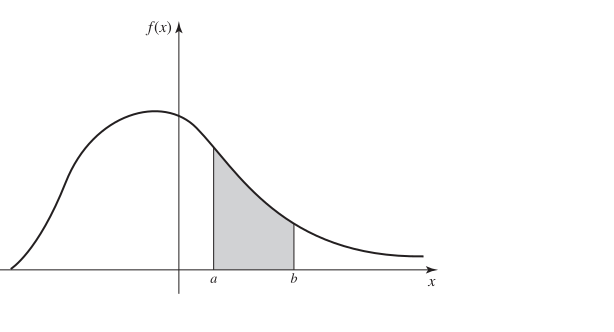
\includegraphics[scale = .3]{Images/PDF_1.png}
\caption{ Here the shaded area is the probability of a random variable $X$ taking value between $a$ and $b$, so this means the shaded area is $\mathbb{P}(X \in [a, b]) = \int_{a}^{b} f(x) dx$}
\end{figure}

\item Now how do we calculate probability of $X$ takes value in the interval $[a, b]$, the idea is we can simply integrate, so $\mathbb{P}(X \in [a, b]) = \int_{a}^{b} f(x) dx$, since integration meas finding area under the curve, so the probability of $X$ takes value in $[a, b]$ = area under the curve in the interval $[a, b]$.


\framebreak

\begin{varblock}{\Thm{Definition} (Probability Density Function (PDF))}

If $X$ is a continuous random variable then a \alert{nonnegative} function $f$ on $\mathbb{R}$ is called the probability density function (in short PDF) of $X$ if for any interval $\mathcal{I}$, we have

\begin{align*}
\mathbb{P}(X \in \mathcal{I})=\int_{\mathcal{I}} f(x) d x
\end{align*}

and it satisfies $\int_{-\infty}^{\infty} f(x) dx = 1$ (the density function should be integrated to $1$).


\end{varblock}


\item For example, for interval $[a, b]$ we can calculate

\vspace*{-.3cm}
\begin{align*}
\mathbb{P}(X \in [a, b]) = \mathbb{P}(a \leq X \leq b)=\int_a^b f(x) d x
\end{align*}



\item Similarly, $\mathbb{P}(X \geq a)=\int_a^{\infty} f(x) d x$ and $\mathbb{P}(X \leq b)=\int_{-\infty}^b f(x) d x$. 


\item We see that the density function $f$ characterizes the distribution of a continuous random variable $X$ in much the same way that the probability mass function characterizes the distribution of a discrete random variable.


\item In this chapter we will see 3 important continuous distributions, 

\begin{itemize}
	\item \emph{Uniform distribution}, 
	\item \emph{Normal distribution} and 
	\item \emph{Exponential distribution} 
\end{itemize}


\item Let's see the uniform distribution now. Notice this is a continuous uniform distribution, the idea is very similar to discrete, but it's for a continuous random variable.

\item Intuitively, a Uniform random variable on the interval $(a, b)$ is a completely random number between $a$ and $b$. Here is the formal definition,

\begin{varblock}{Uniform Distribution}
A continuous random variable $X$ is said to follow the \alert{Uniform Distribution} on the interval $(a, b)$ if its PDF is

$$
f(x)= \begin{cases}\frac{1}{b-a} & \text { if } a<x<b, \\ 0 & \text { otherwise. }\end{cases}
$$

We denote this by $X \sim \operatorname{Unif}(a, b)$.
	
\end{varblock}


\item Let's see a real life example, (this is adapted from \citet{anderson_statistics_2020})

\framebreak

\item Think about a random variable $X$ that represents the flight time of an airplane traveling from Dhaka to Chittagong. Suppose the flight time can be any value in the interval from 60 minutes to 90 minutes. With every 1-minute interval being equally likely, we can think the random variable $X$ follows a uniform probability distribution, so $X \sim \operatorname{Unif}(60, 90)$.

\item Now because $\frac{1}{90 - 60} =  \frac{1}{30}$, the PDF of $X$ can be written as 

\begin{align*}
	f(x) = \begin{cases}
		 \cfrac{1}{30} & \text{ if } 60 \leq x \leq 90, \\
		\\
		0 & \text{ otherwise}
	\end{cases}
\end{align*}

\item  How does it look like?

\begin{figure}[H]
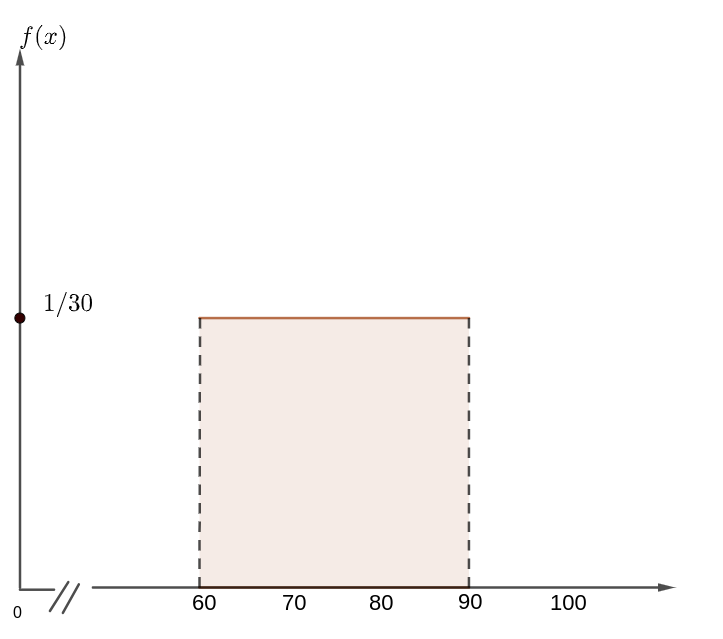
\includegraphics[scale = .2]{Images/Cont_Uniform.png}
	
\end{figure}


\item Now with this density we can calculate the probability of $X$ taking value in any interval, for example, 

\begin{align*}
	\mathbb{P}(X \in [65, 75]) = \int_{65}^{75} f(x) dx = \int_{65}^{75} \frac{1}{30} dx = \frac{1}{30} [x]_{65}^{75} = \frac{1}{30} (75 - 65) = \frac{10}{30} = \frac{1}{3}
\end{align*}

\item So this means there is $1/3$ probability that the flight time will be between 65 minutes and 75 minutes.

\item Note that this also shows probability is an area under the curve, in the following this is the shaded area,

\begin{figure}
 	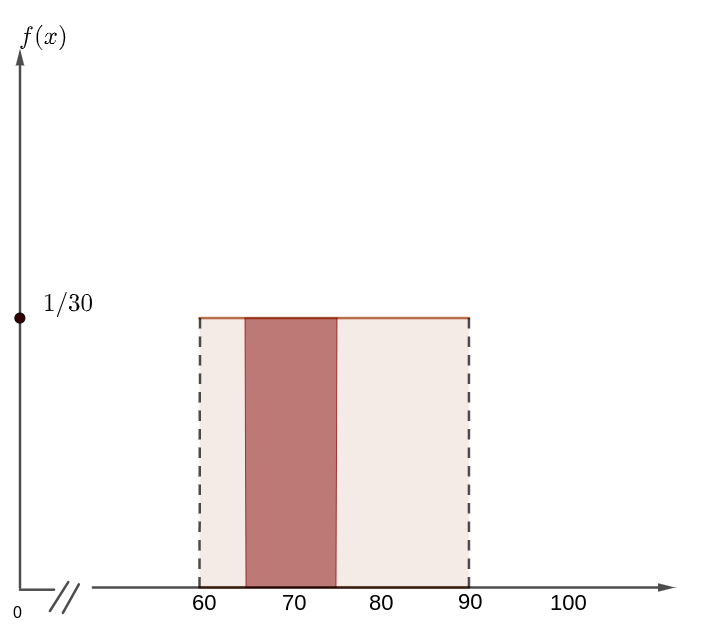
\includegraphics[scale = .2]{Images/Cont_Uniform_area.png}
 \end{figure} 

\item Since in this case the area is a rectangle, we can apply the formula for area of a rectangle to calculate the area, which is $10 \times \frac{1}{30} = \frac{10}{30} = \frac{1}{3}$.


\item Similarly, we can calculate $\mathbb{P}(X \in [70, 80]) = \frac{1}{3}$, $\mathbb{P}(X \in [75, 85]) = \frac{1}{3}$ and so on.


\framebreak

\item Here is another example, suppose we have a random variable $X$ takes value in $[0, 1]$, so $\mathcal{X} = [0, 1]$, with following PDF,

$$
f(x)= \begin{cases}2 x & \text { for } 0<x<1 \\ 0 & \text { otherwise. }\end{cases}
$$

\begin{figure}
	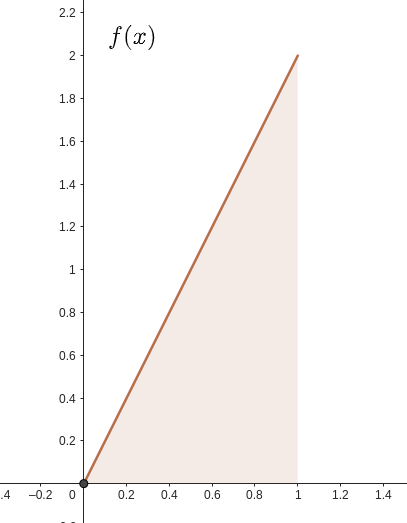
\includegraphics[scale = .25]{Images/cont_pdf.png}
\end{figure}


\item Is this a valid PDF? YES! note it satisfy two conditions

\begin{itemize}
\item $f(x) \geq 0$ for all $x$
\item $\int_{0}^{1} f(x) dx = \int_{0}^{1} 2x dx = 1  $ 
\end{itemize}

\item You should compare and contrast these two conditions with the conditions for a PMF.

\item Can we calculate $\mathbb{P}(X \in [0.5, 0.7]) = ?$ Yes we can...


\begin{align*}
	\int_{0.5}^{0.7} f(x) dx = \int_{0.5}^{0.7} 2x dx = [x^2]_{0.5}^{0.7} = 0.7^2 - 0.5^2 = 0.49 - 0.25 = 0.24
\end{align*}

\item So now we know $\mathbb{P}(X \in [0.5, 0.7]) = 0.24$

\item Note in this case we cannot apply the formula for rectangle, since the area is not a rectangle. Uniform distribution is a special case where we can apply the formula for rectangle, but generally we need to use integration to calculate the area. 

\item so always remember integral = area = probability.



\framebreak

\textbf{Some Important Remarks PDF}

\item When we calculate $f(x)$ for any $x$, \emph{is this a probability, the answer is no}, it's just a function (look at the last example in some points it is more than $1$). So the value of the density function $f(x)$ is not a probability, but it helps to to calculate probabilities when we do integration. {\color{red} Notice! this is an important difference with PMF}: Unlike PMF, any  PDF does not directly give us probabilities, we need to integrate this in a range and then we get a probability. 




\item  Note: We calculated $\mathbb{P}(X \in [a, b]) = \int_{a}^{b} f(x) dx$, then using this you might want to calculate  $\mathbb{P}(X = a) = \int_{a}^{a} f(x) dx$. Clearly this is $0$, since $\int_{a}^{a} f(x) dx = 0$, so we get $\mathbb{P}(X=a)=0$. Now this means for a continuous random variable $X$, for any constant, we will always have $0$ probability. For example $\mathbb{P}(X = 3) = 0$, $\mathbb{P}(X = 100) = 0$ or $\mathbb{P}(X = 3.5) = 0$ and so on.

\item From this you might conclude that \alert{$X=a$ is impossible} because it happens with $0$ probability. But isn't this strange or counter-intuitive? Because if this is impossible then $X$ will not take any value at all, since we will always have $0$ probability.


\item So what is happening here? The last conclusion is actually not correct. It's not that \alert{$X=a$ is impossible} rather what happens here is that the probability $X$ is \alert{spread so thinly} that we fail to calculate it precisely. This is why for a continuous random variable we can only calculate probabilities on any intervals or sets, \emph{NOT for any fixed value}, so we write $\mathbb{P}(X = a) = 0$.


\item {\color{red} Bonus Question:} For a continuous random variable is there any difference between $\mathbb{P}(X \in (a, b))$ and $\mathbb{P}(X \in [a, b])$?  



\end{itemize}

\end{frame}









\subsection{Cumulative Distribution Function - CDF}
\frame{\subsectionpage}

\begin{frame}[allowframebreaks]{Probability Distributions}{CDF for Discrete R.V.}

\begin{itemize}


\item If we know PMF or PDF of a random variable, we can also calculate \emph{cumulative probabilities}. Cumulative Probability means probabilities upto a certain value. 

\item For example, $\mathbb{P}(X \leq 2)$ is a cumulative probability, it means for the random variable $X$ what is the probability of taking value $2$ or less than $2$.

\item For the PMF given in page 25, we can calculate

\begin{align*}
	\mathbb{P}(X \leq 2) &= \mathbb{P}(X = 0) + \mathbb{P}(X =1) + \mathbb{P}(X = 2)\\
	& = f(0) + f(1) + f(2)
\end{align*}


\item Often cumulative probabilities are represented using a function called \emph{cumulative distribution function} in short CDF. CDF is a function defined on the real line, where for any value $x$, it gives the cumulative probability upto that value.

\framebreak

\begin{varblock}{\Thm{Definition } (The cumulative distribution function (CDF))}
	The Cumulative Distribution Function or CDF of of a random variable $X$ is the function $F(x)$ defined as 

\begin{align*}
F(x)=\mathbb{P}(X \leq x), \quad \text{ for } -\infty < x < \infty
\end{align*}
\end{varblock}

\item So the function just gives the cumulative probabilities for each $x \in \mathbb{R}$. For example, using the PMF in page 29, we can easily find the CDF for different $x$. Here we need to find for $0$, $1$, $2$ and $3$

\begin{align*}
	F(0) &= f(0) = 1/8 \\
	F(1) &=  f(0) + f(1) = 4/8 \\
	F(2) &=  f(0) + f(1) + f(2) = 7/8 \\
	F(3) &=  f(0) + f(1) + f(2) + f(3) = 1
\end{align*}

\item We can also think about what happens in the interval $(0, 1)$, note that in this interval $X$ does not take any values, so the cumulative probabilities in this interval is $0$

\item Following is the CDF plot,


\framebreak

\begin{figure}
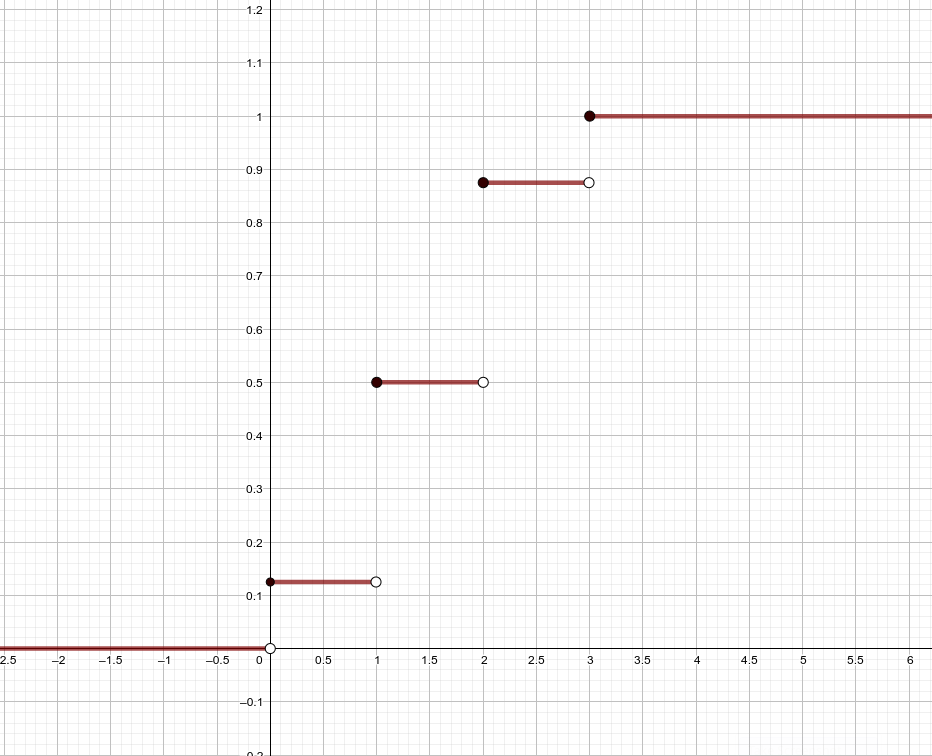
\includegraphics[scale = .3]{Images/CDF.png}
\caption{Notice there is a jump when the random variable takes its value, and the difference where there is a jump is the probability. Also note that the CDF function is defined for the whole $\mathbb{R}$}
\end{figure}

\framebreak

The last figure can be written as a piecewise function

% \begin{columns}
% \begin{column}{0.5\textwidth}
\begin{align*}
F(x)= \begin{cases}0 & : x<0 \\ 
\frac{1}{8} & : 0 \leq x<1 \\ 
\frac{4}{8} & : 1 \leq x<2 \\ 
\frac{7}{8} & : 2 \leq x<3 \\ 
1 & : x \geq 3
\end{cases}
\end{align*}

\medskip

There are $3$ important properties for the CDF, 

\medskip
\begin{itemize}
\item 1) \textbf{Always Non-Decreasing:} If $x_1 \leq x_2$, then $F\left(x_1\right) \leq F\left(x_2\right)$. 
\item 2) \textbf{Right Continuous:} $F(a)=\lim\limits_{x \rightarrow a^{+}} F(x)$.
\item 3) \textbf{At infinity the limits are $0$ and $1$} $\lim\limits_{x \rightarrow-\infty} F(x)=0$ and  $\lim\limits_{x \rightarrow \infty} F(x)=1$.
\end{itemize}

% \end{column}
% \begin{column}{0.5\textwidth}  %%<--- here
% \begin{figure}
% 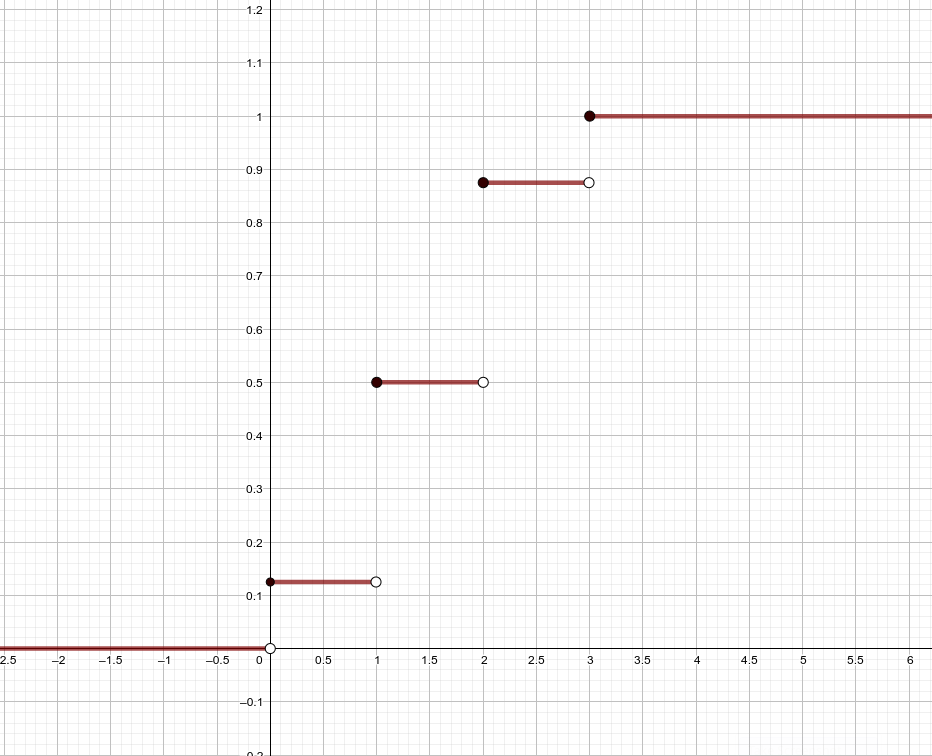
\includegraphics[scale = .2]{Images/CDF.png}
% \caption{Notice there is a jump when the random variable takes its value, and the difference where there is a jump is the probability. Also note that the CDF function is defined for the whole $\mathbb{R}$}
% \end{figure}
% \end{column}
% \end{columns}




% \item \cite{anderson_statistics_2020} motivated the idea of PMF using \alert{empirical discrete distribution}.

% \item The idea is if we know the Population, then we will look for how the values of the random variables are distributed in the population.

% \item Following example will illustrate this idea, this is taken from \cite{anderson_statistics_2020}.


% \item This example gives us a nice intuitive idea, but note that usually we will never know or have access to the population.





\end{itemize}

\end{frame}



\begin{frame}[allowframebreaks]{Probability Distributions}{CDF for Continuous R.V.}

\begin{itemize}
\item  If we know the PDF of a random variable, we can also actually easily calculate the cumulative distribution function or CDF. Notice $\mathbb{P}(X \leq x) = \mathbb{P}(X \in (-\infty, x) )$.

\item Also we can see that $F(x) = \mathbb{P}(X \leq x) = \mathbb{P}(X \in (-\infty, x) ) = \int_{-\infty}^{x} f(t) dt$. Here we used $t$ in PDF because we have $x$ in the limit.

\item CDF is just a function we can find by taking these probabilities. A picture might be helpful here. Here is a PDF, and the associated CDF \footnote[frame]{You can use this nice Wolfram Demonstration, to have a clear idea, click here \url{https://demonstrations.wolfram.com/PercentilesOfCertainProbabilityDistributions/}}

\begin{figure}
\centering
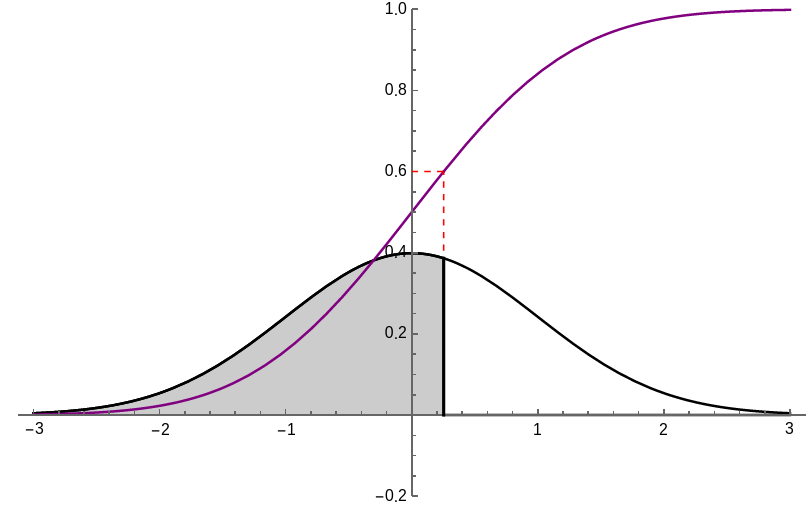
\includegraphics[scale = .25]{Images/PDF_CDF.png}
\caption{The density function $f(x)$ is the Bell-Shaped curve, the shaded are is $\mathbb{P}(X < .253) = \mathbb{P}(X \in (-\infty, .253)) = .60$. The function in the purple color is the cumulative distribution function (CDF) $F(x)$.}
\end{figure}

\item So the CDF or the cumulative distribution function $F(x)$ simply gives us the cumulative probabilities at each $x$.


\item  Once we understand what is cumulative probabilities, we can understand \alert{quantiles} or \alert{percentiles}.

\item In the last figure we showed


\begin{align*}
P ( X \leq 0.253) = F(0.253) = 0.6
\end{align*}

\item In this case we say the number $0.253$ is $0.6^{th}$ \alert{quantile} of the distribution. 

\item Notice this actually means $60\%$ values of the random variable is below $0.253$.

\item We also say $0.253$ is the $60^{th}$ \alert{percentile} of the distribution.

\item So quantiles and percentiles are same things, when it come to quantiles we write in decimals, for example $0.6$, $0.7$, etc. However for percentile we write $60\%$, $70\%$.

\item So if someone asks you what is $65\%$ percentile or $.65^{th}$ quantile of the distribution, you should say this is a value below which there are $65\%$ values of the random variable.




\end{itemize}
\end{frame}


\subsection{Summary Measures - Expectation $\mathbb{E}(\cdot)$ }
\frame{\subsectionpage}

\begin{frame}[allowframebreaks]{Probability Distributions}{Summary Measure - Expectation $\mathbb{E}(\cdot)$}

\begin{itemize}

\item Calculating Expected Value and Expectation is very easy, let's first see the definition of Expectation and we will do an example right away!


\begin{varblock}{\Thm{Definition } (Expected Value)}

If $X$ is a \alert{discrete random variable} with PMF $f(x)$ then the \alert{Expectation}  or the \alert{Expected Value} of $X$ is defined as 

\begin{align*}
\mathbb{E}(X) = \sum_{\text{all values }x} x f(x)
\end{align*}

 If $X$ is a \alert{continuous random variable} whose PDF is $f(x)$ then it is defined as follows:

\begin{align*}
\mathbb{E}(X)=\int_{-\infty}^{\infty} x f(x) d x .
\end{align*}



We will usually use the notation $\mathbb{E}(\cdot)$ to denote that we are performing \alert{Expectation} on $X$.

\end{varblock}

\framebreak


\item So let's break it down ... For a discrete random variable, if we know the PMF, then calculating Expected value is not difficult, it's just multiplying $x$ with $f(x)$ and then adding them altogether. Let's calculate the Expectation for the random variable $X$ from Example 3.1. 

\item Recall the PMF of Example 3.1,


\begin{align}
f(x)= \begin{cases} 1/8 & \text { if } x=0 \\ 
3/8 & \text { if } x=1 \\ 
3/8 & \text { if } x=2 \\ 
1/8 & \text { if } x=3 \\ 
0 & \text { otherwise }\end{cases}
\end{align}

\item So we can calculate the expected value as,

\begin{align*}
\mathbb{E}(X) &= \left(0 \times f(0)\right) + \left(1 \times f(1)\right) + \left(2 \times f(2)\right) + \left(3 \times f(3)\right) \\
&=\left(0 \times 1/8\right) + \left(1 \times 3/8\right) + \left(2 \times 3/8\right) + \left(3 \times 1/8\right) = 1.5
\end{align*}

\item So calculation is very easy, now we may ask \emph{what does expected value mean}?

\item Actually Expectation (or Expected value) is like average, but it is for a population, so it's a \emph{population average} we call it also \emph{population mean}, let's explain how....




\framebreak

\item We will use the Example 3.5 again to understand the idea of Expectation. Suppose here is the population data (you can think about an excel file with $300$ rows)

\begin{align*}
&\underbrace{0, 0, 0, 0, 0, 0, 0, 0, \ldots, 0}_{54 \text{ days so } 54  \text{ rows}}, \underbrace{1, 1, 1, 1, 1, 1, \ldots, 1}_{117 \text{ days so } 117 \text{ rows}}, \underbrace{2, 2, 2, 2, 2, 2, \ldots, 2}_{72 \text{ days so } 72 \text{ rows}}, \underbrace{3, 3, 3, 3, 3, 3, \ldots, 3}_{42 \text{ days so } 42 \text{ rows}}, \\
&\underbrace{4, 4, 4, 4, 4, 4, \ldots, 4}_{12 \text{ days so } 12  \text{ rows}}, \underbrace{5, 5, 5 }_{3 \text{ days so } 3 \text{ rows}}
\end{align*}

\item If someone asks what is the average number of selling in last $300$ days? You might take the average of these numbers and if you do this then the average will be $1.5$.

\item But now using the PMF in page 29, if we calculate the expected value, we will get the same answer,

\begin{align*}
 	& (0 \times f(0))+ (1 \times f(1)) + (2 \times f(2)) + (3 \times f(3)) + (4 \times f(4)) + (5 \times f(5)) \\
 	& = (0 \times 54/300) + (1 \times 117/300) + (2 \times 72/300) + (3 \times 42/300) + (4 \times 12/300) + (5 \times 3/300) \\
 	& = 1.5
 \end{align*} 

\item So the Expected Value or Expectation is actually a population average. It's just we are not doing the average directly, rather we are weighting values with their probabilities. 

\item You may ask why we are learning this formula? What's the benefit?

\item There are at least three reasons why?
\medskip
\begin{itemize}
	\item  First, we don't have to take average of huge number of values, rather we can just use the PMF and calculate the expectation. 

	\item Second, we can calculate the expectation even if we don't have the population data but only know the PMF.

	\item Third, we can extend this idea to continuous case, the idea is replace the $\sum$ with $\int$
\end{itemize}

\item Homework: Can you calculate the expected value of the Discrete Uniform in page $35$, where $X \sim \mathrm{DUnif}\{10, 20, 30 \}$


\item So \emph{Expectation} is the population average, and roughly you can say it's a \alert{central value} such that more probabilities (or weights) are near this value. This is why it is often called a measure for \alert{central tendency}! 

\item Notice for the expected value we calculated 1.5 (page 54, coin toss example) is between $1$ and $2$, and $1$ and $2$ are the two points where the probability is highest for this random variable.


\framebreak

\item Now let's see how to calculate the expected value of a continuous random variable $X$.

\item We do it for the random variable given in page $42$, recall the PDF is given by,

\begin{align*}
f(x)= \begin{cases}2 x & \text { for } 0<x<1 \\ 0 & \text { otherwise. }\end{cases}
\end{align*}

\item We can calculate the expected value (just by \emph{replacing sum with integration!})

\begin{align*}
\mathbb{E}(X) &= \int_{-\infty}^{\infty} x f(x) d x = \int_{0}^{1} x (2x) dx = \int_{0}^{1} 2x^2 dx \quad \ldots \\	
\ldots &= 2 \int_{0}^{1} x^2 dx = 2 \times \left[\frac{x^2}{3}\right]^{^1}_{_{0}} = \frac{2}{3} \times \left[x^3\right]_{0}^{1}  \quad \ldots \\
\ldots &= \frac{2}{3} \times \left[{1^3} - {0^3}\right] = \frac{2}{3} \times 1 = \frac{2}{3} .
\end{align*}


\framebreak

\item Let's do another example. 

\item Let's calculate the expected value of the Uniform distribution where $X \sim \mathrm{Unif}(a, b)$

\begin{align*}
	\mathbb{E}(X) &= \int_{-\infty}^{\infty} x f(x) d x = \int_{a}^{b} x \frac{1}{b-a} dx = \frac{1}{b-a} \int_{a}^{b} x dx = \frac{1}{b-a} \left[\frac{x^2}{2}\right]_{a}^{b} \\
	&= \frac{1}{2(b-a)} \left[x^2\right]_{a}^{b} = \frac{1}{2(b-a)} \left[b^2 - a^2\right]  = \frac{b^2 - a^2}{2(b-a)} = \frac{(b+a)(b-a)}{2(b-a)} = \frac{b+a}{2}
\end{align*}


\item This means Expected value of a Uniformly distributed random variable is the average of the two end points of the interval. This seems very intuitive, since the probability is same for all values, so the expected value should be the average of the two end points. 

\item Question: What is the expected value of the random variable $X$ from the flight example? Recall $X \sim \mathrm{Unif}(60, 90)$



\item \textbf{\color{red}A Notational Remark:}  You should always think about following picture if you think about Expectation of a random variable $X$. Often the constant that we get after calculating the expectation is denoted by $\mu$. So from now on, if you see $\mu$ (although sometimes this is a bit misleading because of normal random variable, we will see it later, but it's been used), you should understand this is an expected value like $1.5$.

\begin{figure}
	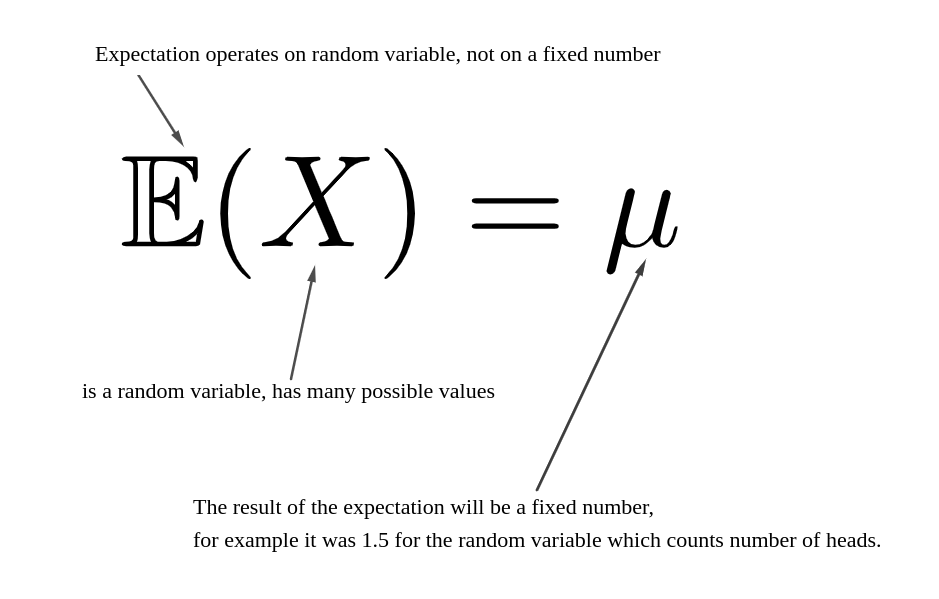
\includegraphics[scale = .3]{Images/Expectation_1.png}
\end{figure}


\item Finally always remember \alert{Population Mean, Expectation, Expected Value}, they are all same thing!




\end{itemize} 


\end{frame}



% \begin{frame}{Summary Measure - Expectation}

%  \begin{itemize}
%     \item So we get this expected value $1.5$, what does this mean?

%     \item Roughly you can interpret this like a \alert{central value} such that more probabilities (or weights) are near this value. This is why this is often called a measure for \alert{central tendency}!


%     \item Another name of Expectation is \alert{Population Mean}, or so often we will say \alert{Population Mean} rather than \alert{Expectation} (why Population?)

%     \item So \alert{Population Mean, Expectation, Expected Value}, they are all same thing!

%     \item Notice $1.5$ is between $1$ and $2$, and $1$ and $2$ are the two points where the probability is highest for this random variable.

%     \item Does this make sense? 


%     \item This is all about Expectation or Expected value of the random variable. 


%     \item Note that in this case, to calculate the Expected value we need to know the PMF (or all the probabilities when $X$ takes different values).


%     \item So if we don't know PMF then we cannot calculate expectation.

%     \item \textbf{\color{red}A notational remark:} Often the constant that we get after calculating the expectation is denoted by $\mu$. So from now on, if you see $\mu$, you should understand this is an expected value like $1.5$.

%     \item Now let's see about variance.

%   \end{itemize} 


% \end{frame}

\subsection{Summary Measures -  Variance $\mathbb{Var}\mathrm{ar}(\cdot)$ }
\frame{\subsectionpage}

\begin{frame}[allowframebreaks]{Discrete Probability Distributions}{Summary Measure - Variance $\mathbb{Var}\mathrm{ar}(\cdot)$}

\begin{itemize}
\item Like Expectation, variance is also a summary measure, where the expectation gives an idea of the central value, variance gives the idea how \alert{dispersed the values are}. 


\begin{varblock}{\Thm{Definition } (Variance)}

If $X$ is a discrete random variable with PMF $f(x)$ then the \alert{Variance} of $X$ is defined as 

\begin{align*}
\Var(X) = \mathbb{E}\left( \left(X - \mathbb{E}\left(X\right)\right)^2 \right) = \mathbb{E}\left( \left(X - \mu \right)^2 \right) = \sum_{\text{all values } x}(x-\mu)^2 f(x)
\end{align*}

If $X$ is a continuous random variable with PDF $f(x)$, then the \alert{Variance} of $X$ is defined as 

\begin{align*}
\Var(X) = \mathbb{E}( (X-\mu)^2) =\int_{-\infty}^{\infty} (x-\mu)^2 f(x) d x .
\end{align*}
	
\end{varblock}

\item First note that, Variance is also an Expectation, but it is an \alert{Expectation of $\left(X - \mu \right)^2$}, NOT $X$. 

\item So what is $\left(X - \mu \right)^2$? Or what is $\left(X - \mu \right)$? Ans: $X - \mu$ is the deviation of the random variable from its Mean and $\left(X - \mu \right)^2$ is the squared deviation.

\item So variance is the Expectation of the squared deviation.

\item Let's calculate $\Var(X)$ for the random variable $X$, which counts the number of heads (PMF in page 27).

\begin{align*}
\Var(X) &= \left( \left(0 - 1.5\right)^2 \times f(0)\right) + \left( \left(1 - 1.5\right)^2 \times f(1)\right) + \\
& \qquad \left( \left(2 - 1.5\right)^2 \times f(2)\right) + \left( \left(3 - 1.5\right)^2 \times f(3)\right) \\
& = \left( \left(-1.5\right)^2 \times 1/8\right) + \left( \left(-0.5\right)^2 \times 3/8\right) + \left( \left(0.5\right)^2 \times 3/8\right) + \left( \left(1.5\right)^2 \times 1/8\right)\\
&=\left(2.25 \times 1/8\right) + \left(0.25 \times 3/8\right) + \left(0.25 \times 3/8\right) + \left(2.25 \times 1/8\right) \\
&= 0.75
\end{align*}

\item So calculating Variance is really easy, if we know PMF we can easily calculate the variance. 

\item The interpretation of the variance is how dispersed the values are.

\item \textbf{\color{red}A Notational remark:} Often the constant that we get after calculating the variance is denoted by $\sigma^2$. So from now on, if you see $\sigma^2$, you should understand this is a variance like $.75$.

\item The square root of the variance is called \alert{Standard Deviation}, so if $\sigma^2$ is the Variance, then $\sigma$ is the standard deviation.



\item Like discrete random variables we can also calculate Expected values and Variance for a continuous random variable.

\item The expectation and the variance of a continuous random variable can be calculated the same way we did for discrete, however, we need \alert{Integration} here (DIY \faEdit \faEdit \faEdit)



\end{itemize} 


\end{frame}



% \begin{frame}{Distribution, Mean and Variance}

% \begin{itemize}

% \item Before we proceed further let's summarize what we did so far.

% \item So we had a discrete random variable $X$ which takes values $0, 1, 2, 3$ and it has following PMF,

% \vspace*{-.3cm}
% \begin{align}
% f(x)= \begin{cases} 1/8 & \text { if } x=0 \\ 
% 3/8 & \text { if } x=1 \\ 
% 3/8 & \text { if } x=2 \\ 
% 1/8 & \text { if } x=3 \\ 
% 0 & \text { otherwise }\end{cases}
% \end{align}

% \item PMF tells us about the distribution, because it tells about $\mathbb{P}(X = 0), \mathbb{P}(X = 1), \mathbb{P}(X = 2)$ and $\mathbb{P}(X = 3)$.

% \item But distribution is often too much information, and maybe sometimes we just one or two numbers to understand about the distribution of a random variable. This is what the job of Mean and Variance of the distribution.

% \item Where Mean of the distribution gives us an idea about the central point, the Variance tells us how spread the distribution is, and Standard deviation is just the square root of the Variance.

% \item For this random variable $\mathbb{E}(X) = 1.5$ and $\Var(X) = .75$, and standard deviation is $\sqrt{.75}$.



% \end{itemize} 


% \end{frame}


\section{Parametric Family of Probability Distributions}
\frame{\sectionpage}


\subsection{Discrete Distribution - Bernoulli and Binomial Distribution}
\frame{\subsectionpage}



\begin{frame}[allowframebreaks]{Bernoulli \& Binomial Random Variables}





\begin{itemize}

\item If a random variable $X$ has only two values $0$ and $1$, we call the random variable a \alert{Bernoulli Random variable}, and its distribution is known as \alert{Bernoulli distribution},  some examples, 

\begin{itemize}
\item Random Experiment - Toss a coin. Random Variable $X = 1$ means head, $X = 0$ means tail.

\item Random Experiment - Pick a random person from a Population of people. Random Variable $X = 1$ means female, and $X = 0$ means male 

\item Random Experiment - Calling a customer.  Random Variable $X = 1$ means picked up the call, $X = 0$ means didn't pickup.

\end{itemize}

\item In practice or in real life scenario, when you have possible data with $0, 1, 0, 1, 0, 1$, you can think about these are values of some Bernoulli random variables. So in any experiment, when we have only two possible outcomes we can think about a modeling that experiment using a Bernoulli random variable. For a Bernoulli random variable, if $X = 1$, we often call it \emph{``success''} and if $X = 0$, we often call it ``failure''. Here is the formal definition.

\begin{varblock}{\Thm{Definition } (Bernoulli Distribution)}
 \Thm{Definition } (Bernoulli distribution). A random variable $X$ is said to have the Bernoulli distribution with parameter $p$ (we wrote $X \sim \operatorname{Bernoulli}(p)$), if $\mathbb{P}(X=1)= p$ and $\mathbb{P}(X=0)= 1-p$. The PMF of $X$ can be written as,

\begin{align*}
f(x; p) &= p^x {(1 - p)}^{1-x}, \quad \text{ when } x = 0, 1 \\
&  = 0, \quad \text{otherwise}
\end{align*}

where $0<p<1$
\end{varblock}



\item Note that, because of this PMF, we have $\mathbb{P}(X=1)=f(1) = p$ and $\mathbb{P}(X=0)= f(0) = 1-p$.

\item Notice, the parameter $p$ controls the probability and hence controls the distribution of the random variable. For example, if $X \sim \operatorname{Bernoulli}(.3)$, this automatically means $\mathbb{P}(X = 1) = 0.3$ and $\mathbb{P}(X = 0) = 0.7$. Here is how the PMF will look like for different parameters $p$,

\begin{figure}
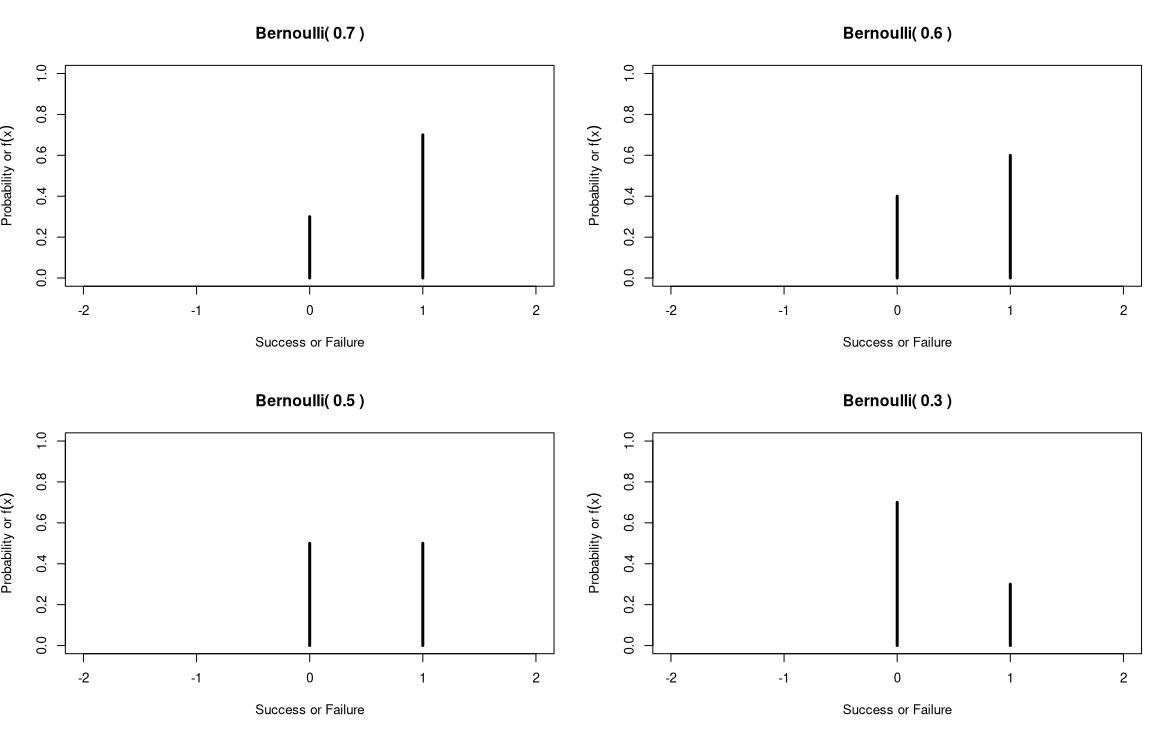
\includegraphics[scale = .3]{Images/BernoulliDistPMF.png}
\end{figure}


\item Because we have the PMF we can also calculate the Expected Value and Variance of a Bernoulli random variable.

\item If you do the calculation, then you should get $\mathbb{E}(X) = p$ and $\Var(X) = p (1-p)$ (please do the calculation!)

\framebreak

\item The Binomial distribution comes when we perform \emph{$n$ independent Bernoulli experiment}.

\item Here is the story - Suppose now we perform $n$ independent Bernoulli experiments (or Bernoulli trials) with parameter $p$. If $X$ is a random variable which represents the total number of success out of the $n$ trials, then we say the random variable $X$ follows Binomial distribution with parameter $n$ and $p$.

\item You already know the example, if we toss a single coin and represent $X$ as a Bernoulli random variable which can take values $1$ (success) or $0$ (failure) with probability $p$, then when we toss $n = 3$ independent coins and represent $X$ as total number of heads (total number of success), then $X$ is said to follow Binomial with parameter $n = 3$ and probability $p$.


\begin{varblock}{\Thm{Definition } (Binomial Distribution)}
	Suppose that $n$ independent Bernoulli trials are performed, each with the same success probability $p$. Let $X$ be the number of successes. The distribution of $X$ is called the Binomial distribution with parameters $n$ and $p$. We write $X \sim \operatorname{Bin}(n, p)$ to mean that $X$ has the Binomial distribution with parameters $n$ and $p$, where $n$ is a positive integer and $0<p<1$. The PMF of $X$ can be written as 

\begin{align*}
f(x; n, p)&=\left(\begin{array}{l}
n \\
x
\end{array}\right) p^x(1-p)^{n-x} \quad \text{ for } x = 0, 1, 2, \ldots, n \\
&= 0, \text{ otherwise}
\end{align*}
\end{varblock}


\item Notice here $x$ is the value of the random variable where $x$ can be $0, 1, 2, \ldots, n$. The PMF looks very similar to Bernoulli PMF, except we have a combination term, recall $\left(\begin{array}{l}
n \\
x
\end{array}\right) = \Combine[n]{x} = \frac{n!}{x! (n-x)!}$. Question is why is this coming? 


\item Here is a short answer, the experiment consisting of $n$ independent Bernoulli trials produces a sequence of successes and failures. The probability of any specific sequence of $x$ successes and $n-x$ failures is $p^x(1-p)^{n-x}$. There are $\Combine[n]{x}$ such sequences.



\item We can also calculate the Mean and the Variance of the Binomial distribution. \alert{If $X \sim \textrm{Bin}(n, p)$, then $\mathbb{E}(X) = np$ and $\Var(X) = np(1-p)$}, where do we get this? You can see the proof in the next page. However there is an easy trick that is you remember Binomial is the sum $n$ independent Bernoulli trials (Let's do it using easy trick!)

\framebreak


\item If $X \sim \mathrm{Bin}(n, p)$, then applying the formula for Expectation

$$
\mathbb{E}(X)=\sum_{x=0}^n x f(x)=\sum_{x=0}^n x\left(\begin{array}{l}
n \\
x
\end{array}\right) p^x q^{n-x} .
$$

\item Note here we wrote $q = (1-p)$. Also note that we have $x\left(\begin{array}{c}n \\ x\end{array}\right)=n\left(\begin{array}{c}n-1 \\ x-1\end{array}\right)$, so
$$
\begin{aligned}
\sum_{x=0}^n x\left(\begin{array}{l}
n \\
x
\end{array}\right) p^x q^{n-x} &=n \sum_{x=0}^n\left(\begin{array}{c}
n-1 \\
x-1
\end{array}\right) p^x q^{n-x} \\
&=n p \sum_{x=1}^n\left(\begin{array}{c}
n-1 \\
x-1
\end{array}\right) p^{x-1} q^{n-x} \\
&=n p \sum_{j=0}^{n-1}\left(\begin{array}{c}
n-1 \\
j
\end{array}\right) p^j q^{n-1-j} \\
&=n p .
\end{aligned}
$$

Then \emph{we get $\mathbb{E}(X) = np$, similarly we can derive the variance is $\mathbb{V}\mathrm{ar}(X) = np(1-p)$ (I am skipping the proof). Again the easy trick is to apply Binomial - Bernoulli relation}.


\item Here is how the PMF will look like for two Binomial distributions, with same $n = 3$ but different $p$.

\begin{figure}
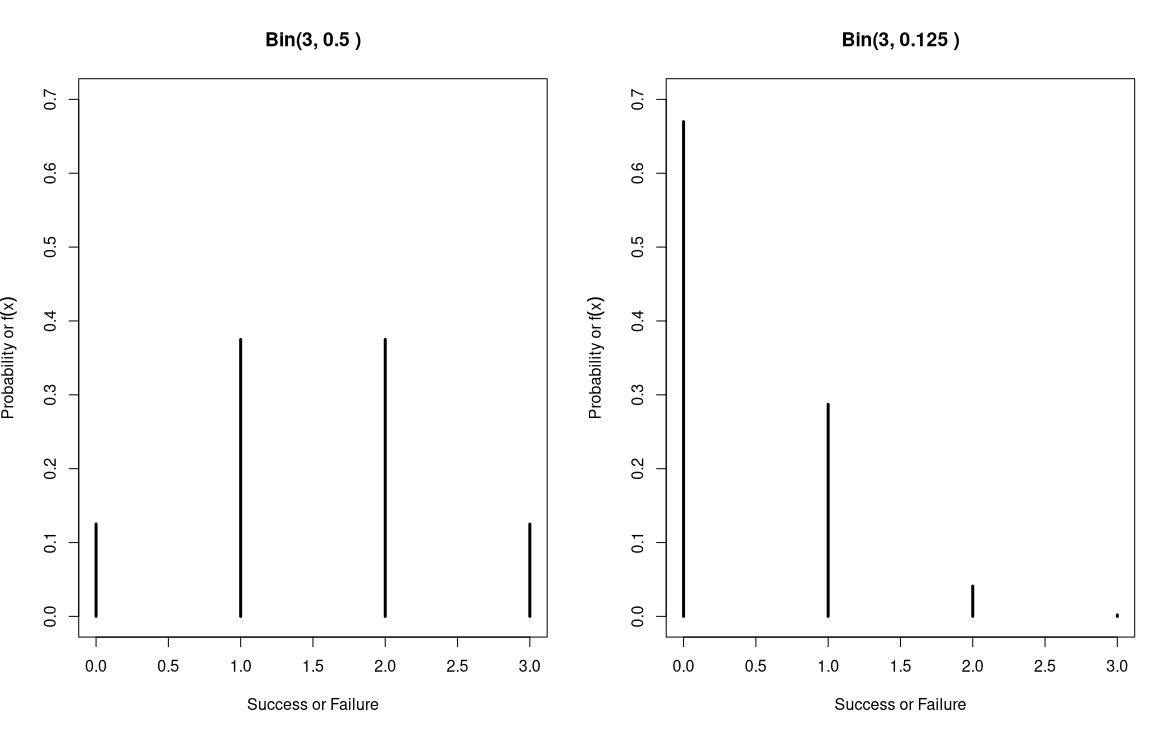
\includegraphics[scale = .3]{Images/Binomial-1.png}
\caption{On the left we have the PMF of $X \sim \textrm{Bin}(3, 0.5)$ and on the right we have $X \sim \textrm{Bin}(3, 0.125)$.  }
\end{figure}



\begin{figure}
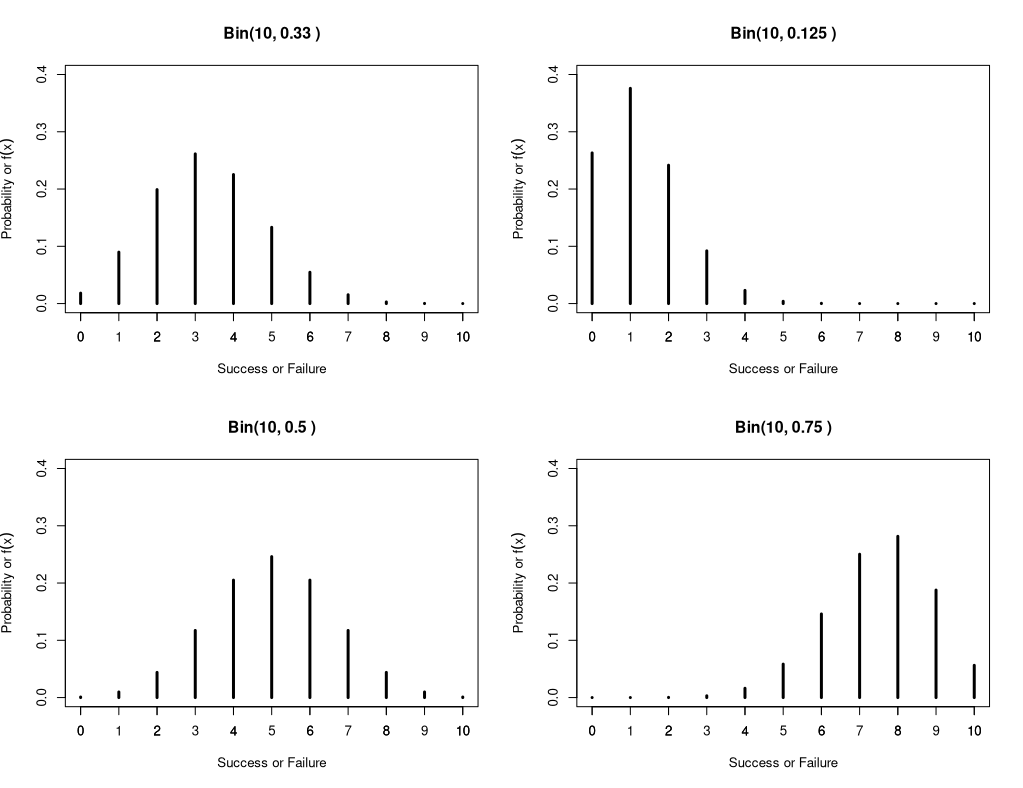
\includegraphics[scale = .3]{Images/Binomial-2.png}
\caption{From top left, we have the PMF of $X \sim \textrm{Bin}(10, 0.33)$, then right $X \sim \textrm{Bin}(10, 0.125)$, then bottom left $X \sim \textrm{Bin}(10, 0.5)$ and right $X \sim \textrm{Bin}(10, 0.75)$  }
\end{figure}


\item Binomial distribution comes in many forms in real life, you should always remember the essential structure - \emph{that is tossing $n$ independent coins and then the random variable is the number of success out of $n$}.

\item Here are some examples where we can think about a Binomial random variable.

\begin{itemize}
\item  Random experiment: Calling $n$ people. Random variable $X$ will represent how many people will answer the call.

\item Random experiment: $n$ students registered for a course. Random variable $X$ will represent how many students will finish it.

\item Random experiment: Randomly asking $5$ people whether they are satisfied with the transportation system of Bangladesh. Random variable is number of people who said "yes"! 

\item And there are more examples in \cite{anderson_statistics_2020}.


\end{itemize}

\item Notice two important assumptions for the Binomial random variable is, 1) all trials are independent and 2) all trials happens with same probability. Only in these cases you can think about the random variable is Binomial.



\end{itemize}


\end{frame}



\subsection{Discrete Distribution - Poisson Distribution}
\frame{\subsectionpage}



\begin{frame}[allowframebreaks]{Poisson Distribution}


\begin{itemize}
\item Now we will consider another distribution known as Poisson distribution. 

\item The situation when you can use Poisson distribution is very similar to Binomial distribution, but the difference is in Binomial you have often a small number of trials, but in Poisson you may have many (in theory infinite) independent trials, with success probability very small.

\item For example, the number of arrivals at a car wash in one hour, the number
of repairs needed in 10 miles of highway, or the number of leaks in 100 miles of pipeline (these examples are from \citet*{anderson_statistics_2020}). Notice, $n$ can be very large, often there is no upper limit, and also the values $x$ also has no upper limit, so it can be $0, 1, 2, 3, \ldots$.


\begin{varblock}{\Thm{Definition } (Poisson Distribution)}
An random variable $X$ has the Poisson distribution with parameter $\lambda$ if the $\mathrm{PMF}$ of $X$ is

\begin{align*}
f(x; \lambda) = \frac{e^{-\lambda} \lambda^x}{x !}, \quad x=0,1,2, \ldots
\end{align*}


We write this as $X \sim \operatorname{Pois}(\lambda)$.	
\end{varblock}


\item This is a valid PMF because we can show that $\sum_{x=0}^{\infty} \frac{\lambda^x}{x !}=e^{\lambda}$.

\framebreak

\item How does Poisson PMF come? The idea is we can think Poisson distribution is a \emph{limiting case} (or limit) of Binomial distribution. More specifically we need $n \to \infty$ and $p \to 0$, then Binomial PMF will converge to Poisson PMF.

\item This means starting from $    \left(\begin{array}{l}
n \\
x
\end{array}\right) p^x(1-p)^{n-x}$ and we take   $n \to \infty$  and $p \to 0$  we get  $\frac{e^{-\lambda} \lambda^x}{x !}$


\item It's a mathematical problem with limit, so we will avoid it, but you should understand that Poisson distribution appears as a limit of Binomial.

\framebreak

\item In real life context it  is often used in situations where we are counting the number of successes in a particular region or interval of time, and there are a large number of trials, each with a small probability of success. The random variable $X$ is again the number of success and but in this case number of success can be $0, 1, 2, 3, \ldots $.

\item Here are some more examples, 

\begin{itemize}
	\item The number of emails you receive in an hour. There are a lot of people who could potentially email you in that hour, but it is unlikely that any specific person will actually email you in that hour.

	\item The number of earthquakes in a year in some region of the world. At any given time and location, the probability of an earthquake is small, but there are a large number of possible times and locations for earthquakes to occur over the course of the year. 

\end{itemize}


\item There are more example in \cite{anderson_statistics_2020}.

\item If $X \sim \mathrm{Pois}(\lambda)$, then we can again calculate (skip the proof)

\begin{align*}
\mathbb{E}(X) = \lambda \quad \text{ and } \quad \Var(X) = \lambda
\end{align*}



\item Here $\lambda$ is the parameter, which is also the mean or expected value. It is often it is called the \emph{rate of occurrence} in the rare events.


\framebreak

\item There are other discrete distributions, e.g., Geometric and Negative Binomial, which we won't cover here. If you are interested to read about them you can read \cite{degroot_probability_2012}.

\end{itemize}


\end{frame}

\subsection{Continuous Distribution - Normal Distribution}
\frame{\subsectionpage}


\begin{frame}[allowframebreaks]{Normal Distribution}

\begin{itemize}

\item We already saw one continuous distribution, which is Uniform distribution, now we will see another one, known as \alert{Normal distribution}.

\item \alert{Normal distribution} is possibly one of the most important continuous probability distributions of all time.

\item   When a random variable $X$ is normally distributed then we write $X \sim \mathcal{N}(\mu, \sigma^2)$. Here $\mu$ and $\sigma^2$ are the \alert{two parameters} of the distribution, which controls the shape of the density function $f(x)$. The density of the normal distribution looks like following.


\begin{figure}
\centering
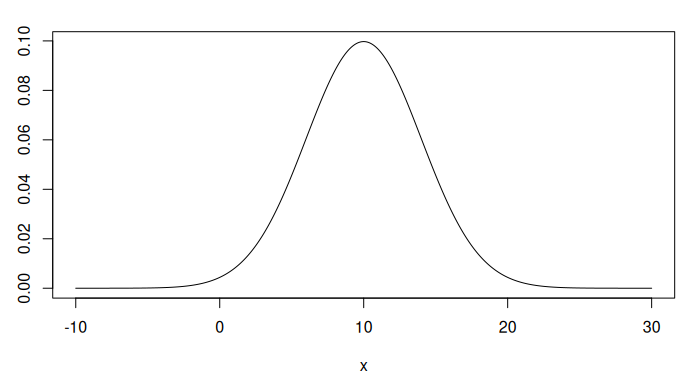
\includegraphics[scale = .4]{Images/pdfNormal_1.png}
\caption{density function of a normal distribution when $\mu = 10$ and $\sigma^2 = 16$}
\end{figure}

\item What is the algebraic form of this function? Here it is

\begin{align*}
f\left(x ; \mu, \sigma^2\right)=\frac{1}{\sqrt{2 \pi \sigma^2}} e^{-\frac{1}{2}\left(\frac{x-\mu}{\sigma}\right)^2}
\end{align*}



\item Since we plotted the density in Figure 10 when $\mu = 10$ and $\sigma^2 = 16$, so this means the density function in Figure 8 is, 

\begin{align*}
f(x; 10, 16) = \frac{1}{\sqrt{2 \pi \times 16}} e^{-\frac{1}{2}\left(\frac{x-10}{4}\right)^2}
\end{align*} 


\item   The range of a normal distributed random variable is the whole real line or $\mathbb{R}$. This means it takes values from $\infty$ to $+\infty$. 


\item $\mu$ is often called the \alert{location} parameter and $\sigma^2$ is called the \alert{dispersion} parameter (why this name, we will see in a minute)


\item Again notice this is a function of $x$, but we also wrote the two parameters $\mu, \sigma^2$ after ``$;$'', always remember when we think about a density function now it's a function of $x$ (this is similar to PMF) but we will write parameters to show that these parameters controls the function. 


\item We can use the density function to calculate the probabilities. Recall probability in this case is the area under the curve within some interval, right?

\item For example, following is a density function with parameters $\mu = 0$, $\sigma^2 =1$, so the function is   $f(x; 0, 1) = \frac{1}{\sqrt{2 \pi}} e^{-\frac{1}{2}x^2}$.


\begin{figure}
\centering
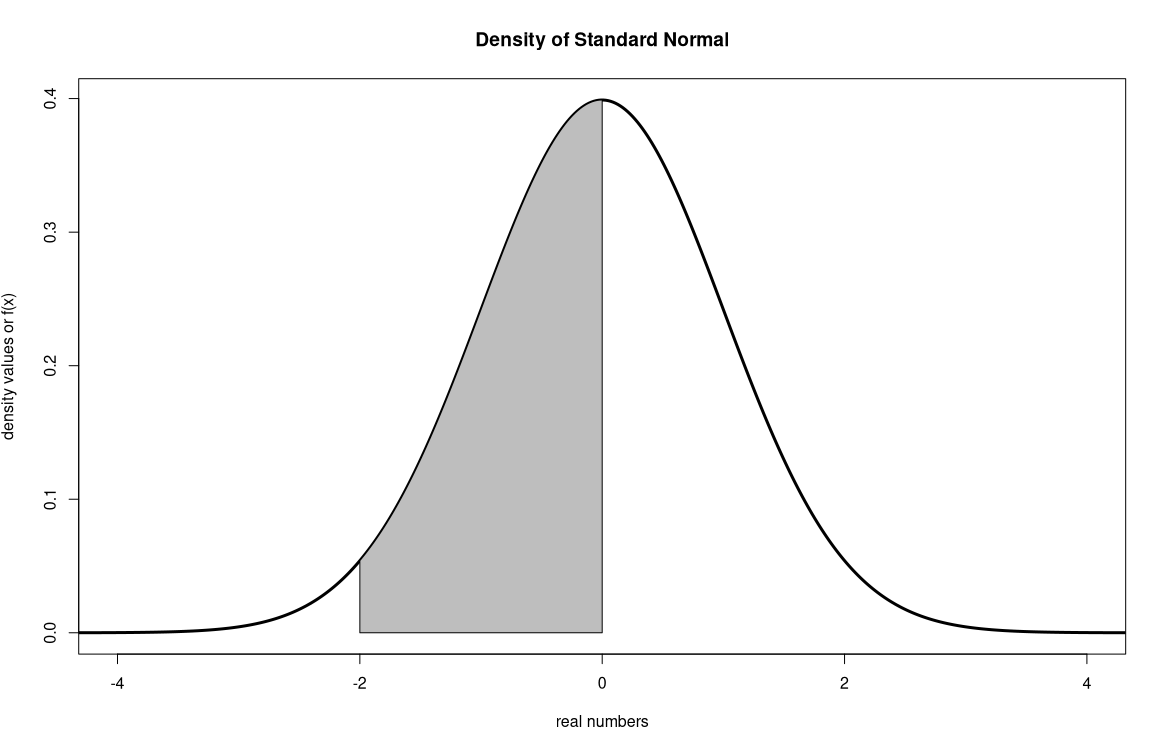
\includegraphics[scale = .25]{Images/Normal_density_area.png}
\caption{This is a density function of a normal distribution with $\mu = 0$, and $\sigma^2 = 1$. The shaded are is a probability, this is $\mathbb{P}(X \in(-2,0))=\int_{-2}^0 f(x; 0, 1) d x=0.4772499$}
\end{figure}




\item Notice for each combination of $\mu$ and $\sigma^2$, we will get a different density function, this means different probability distribution (why?.

\item Why we call them \alert{location} and \alert{dispersion} parameter. This is because If we change $\mu$ and $\sigma^2$, then we can shift the location of the density and also change the spread of the density.

\begin{figure}
\centering
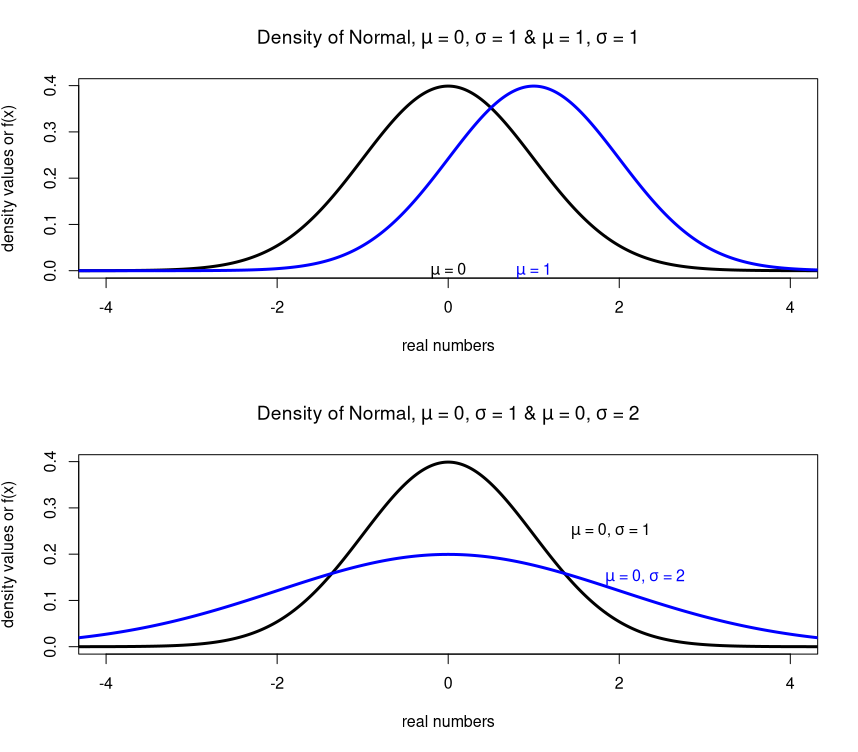
\includegraphics[scale = .3]{Images/Normal_density_parameter_change.png}
\caption{Effect of changing $\mu$ and $\sigma^2$ on the density function.}
\end{figure}

\item So for each combination of $\mu$ and $\sigma^2$, we will get a different density function. Recall we use the density function to calculate different probabilities. So density change is equivalent to distribution change.

\framebreak


\item Normal distribution has some amazing properties, even if you cannot remember the crazy looking density function, you should always remember these properties.

\begin{itemize}
\item If $X \sim \mathcal{N}(\mu, \sigma^2)$ We can calculate the Expected value and Variance. We will get $\mathbb{E}(X) = \mu$ and $\Var(X) = \sigma^2$.

\item Notice the figure the Mean (or expected value) will be always at the center of the Normal distribution. 

\item Then you should remember following picture (this is taken from \cite{anderson_statistics_2020})
\medskip

\end{itemize}

\item[]

\begin{itemize}
\item[]

\begin{figure}
\centering
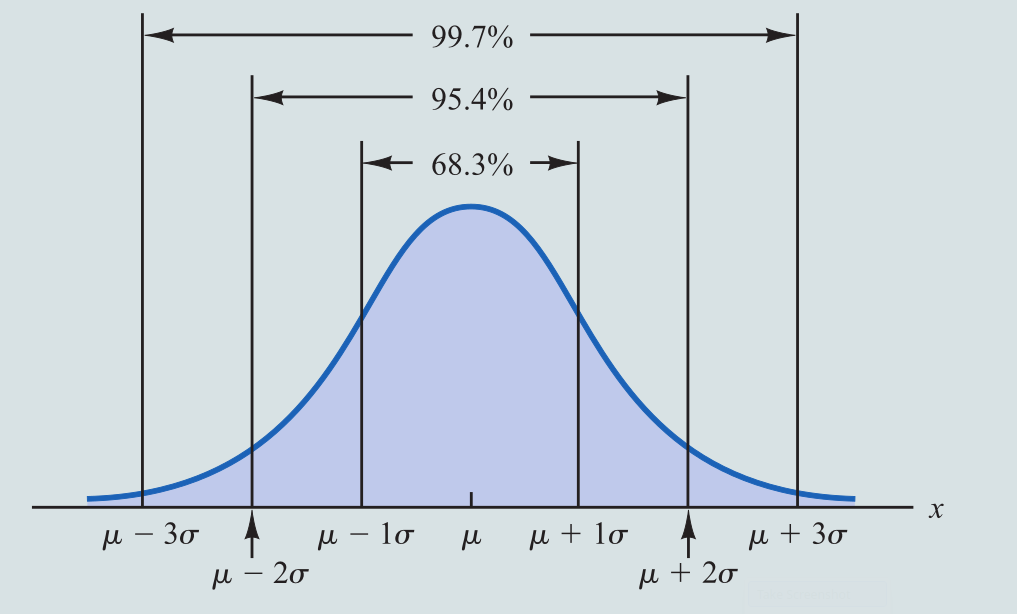
\includegraphics[scale = .25]{Images/PDF_Normal_percentiles.png}

\end{figure}
\end{itemize}

\item This means if we know the mean $\mu$ and variance $\sigma^2$, then we can figure out 

\begin{itemize}
\item   the two points $\mu + \sigma$,  $\mu - \sigma$, and we know that within these two points there will be $68.3\%$ probability. 
\item   the two points $\mu + 2\sigma$,  $\mu - 2\sigma$, and we know that within these two points there will be $95.4\%$ probability. 
\item   the two points $\mu + 3\sigma$,  $\mu - 3\sigma$, and we know that within these two points there will be $99.7\%$ probability. 

\end{itemize}



\item Finally if we know the random variable $X \sim \mathcal{N}(\mu, \sigma^2)$, then we can transform this random variable and get a new random variable $Z$, by

\begin{align*}
Z = \frac{X - \mu}{\sigma}
\end{align*}

\item This what we call \alert{$Z$-transformation, or standardization or normalization}.

\item The interesting thing is it can be proven that $Z \sim \mathcal{N}(0, 1)$.

\item This is sometimes very helpful because we can go back and forth from $\mathcal{N}(\mu, \sigma^2)$ to $\mathcal{N}(0, 1)$.


\item I think now we are ready to do some problems in \cite{anderson_statistics_2020}, we will use the standard normal table at the back of the book 

\end{itemize}


\end{frame}




\subsection{Continuous Distribution - Exponential Distribution}
\frame{\subsectionpage}


\begin{frame}{Exponential Distribution}



\end{frame}


\section{Rules of Expectation and Variance}
\frame{\sectionpage}


\begin{frame}[allowframebreaks]{Rules of Expectation and Variance}

\begin{itemize}
\item We already saw the way to calculate the Expected value\footnote[frame]{Recall we call it also mean or expectation.} of a random variable $\mathbb{E}(X)$, when $X$ is discrete or continuous. Here are the two formulas again

\begin{align*}
\mathbb{E}(X) &= \sum_{\text {all values } x} x f(x) \quad \text{ [when $X$ is discrete]}\\
\mathbb{E}(X) &=\int_{-\infty}^{\infty} x f(x) d x \quad \text{ [when $X$ is continuous]} 
\end{align*}


\item The Variance is also an expectation, but it's the expectation of the squared deviation from mean.

\vspace*{-.3cm}
\begin{align*}
\Var(X) &= \mathbb{E} \left(  \left( X - \mathbb{E}(X) \right)^2 \right)=  \sum_{\text {all values } x} (x - \mathbb{E}(X) )^2  f(x) \quad \text{ [when $X$ is discrete]} \\
\Var(X) &= \mathbb{E} \left(  \left( X - \mathbb{E}(X) \right)^2 \right)= \int_{-\infty}^{\infty}  (x - \mathbb{E}(X) )^2  f(x) dx  \quad \text{ [when $X$ is continuous]}
\end{align*}

\item Always remember! The expected value of a random variable is a constant, so $\mathbb{E}(X) = \text{ constant number }$. Sometimes we write this constant number with $\mu$ regardless of the fact that $X$ follows normal distribution or not. This is not a good notation, but people generally use it.

\bigskip

\item Again you should always keep the following picture in your mind, that expectation works on random variables, not on number, and the result of Expectation is a constant.


\begin{figure}
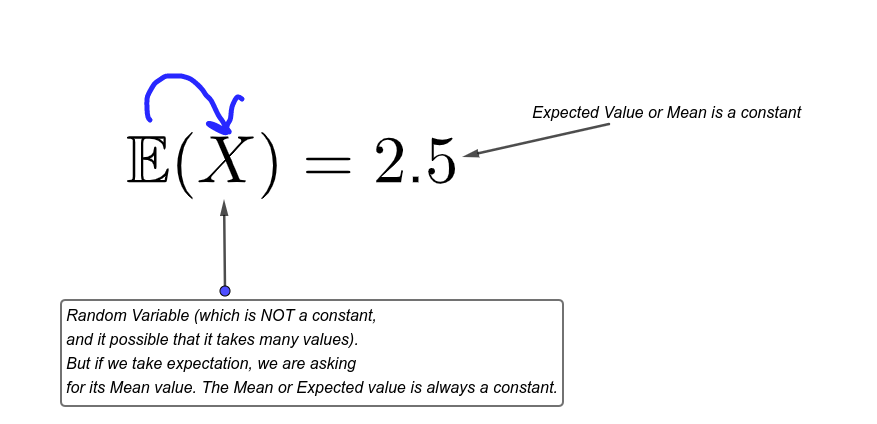
\includegraphics[scale = .5]{Images/RV_1.png}
\end{figure}




\item Now we consider a slightly different problem, we ask what is 

{\huge{
\vspace*{-.5cm}
\begin{align*}
\mathbb{E}(X^2) \text{ or } \mathbb{E}(X^3)  \text{ or } \mathbb{E}(2X + 3) \text{ ??? }
\end{align*}
}}

\item Note that $X^2$, $X^3$ or $2X + 3$ are all functions of random variable $X$. 

\item So our question is for a function $g(X)$, where $g(X)$ can be $X^2$, $X^3$ or $2X + 3$, what is $\mathbb{E}(g(X))$?

\item First of all note that $g(X)$ is also a random variable. So a function of a random variable is also a random variable.

\item It turns out that (we are avoiding the formal proof) in this case we can calculate $\mathbb{E}(g(X))$ by using the distribution of $X$. 

\item So this means ....

\begin{align*}
\mathbb{E}(g(X)) &= \sum_{\text {all values } x} g(x) f(x) \quad \text{ [when $X$ is discrete]}\\
\mathbb{E}(g(X)) &=\int_{-\infty}^{\infty} g(x) f(x) d x \quad \text{ [when $X$ is continuous]} 
\end{align*}

\item Now we can apply this rule more or less for any function $g()$. This rule has an interesting name, it is called - \alert{Law of the unconscious Statistician} or in short \alert{LOTUS} (why this name?)

\item We have already applied LOTUS previously,

\begin{itemize}
\item Calculating variance is an application of this rule, because we are doing $\mathbb{E}\left( \left( X - \mu  \right)^2  \right)$. Here $g(X) =  \left( X - \mu  \right)^2 $.

\item Also in PS-3 when we calculated $\mathbb{E}\left( X^2  \right)$, we have applied LOTUS, here $g(X) = X^2$.

\item You can create more examples, but application of LOTUS is easy!
\end{itemize}

\item So LOTUS is one rule for expectation, there are two other rules for expectation, and we can use LOTUS to prove the following rules,

\begin{itemize}
\item $\mathbb{E}(a) = a$, where $a$ is any constant.
\item $\mathbb{E}(bX) = b \mathbb{E}(X)$, where $b$ is any constant.
\item So together we have $\mathbb{E}(a + bX) = a + b \mathbb{E}(X)$
\end{itemize}

\item The last rule is sometimes called the \alert{linearity of expectation}.


\item We will see the proof for a discrete random variable $X$ with values $x_1, x_2, x_3, \ldots, x_n$.



\begin{align}
\mathbb{E}[a+b X] &=\left(a+b x_1\right) f(x_1) + \left(a+b x_2\right) f(x_2)+ \ldots, +\left(a+b x_n\right) f(x_n) \\
&=\sum_{j=1}^{n}\left(a+b x_i\right) f(x_i) \\
&=\sum_{j=1}^{n} a  f(x_i) + \sum_{j=1}^{n}\left(b x_i\right) f(x_i) \\
&=a \sum_{j=1}^{n} f(x_i)+b \sum_{j=1}^{n} x_i f(x_i) \\
&=a+b \mathbb{E}[X]
\end{align}

\begin{itemize}

\item At (4) we applied the formula for expectation
\item At (5) we just wrote with summation
\item At (6) summation can be separated
\item At (7) take the constant out from summation (this is a rule for summation, see below)
\item At (8) $\sum_{j=1}^{n} f(x_i) = 1$ because this is a PMF, and $\sum_{j=1}^{n} x_i f(x_i) = \mathbb{E}(X)$

\end{itemize}



\item When it comes to summation you can always apply following rules, 

\item 1. $\sum_{i=1}^n a=n a$, where $a$ is constant. For example, $\sum_{i=1}^4 3=4 \cdot 3=12$.
\medskip
\item 2. $\sum_{i=1}^n b x_i = b \sum_{i=1}^n x_i$, where $b$ is a constant.
\medskip
\item 3. $\sum_{i=1}^n\left(a+b x_i\right)=n a+b \sum_{i=1}^n x_i$, where $a$ and $b$ are constants and where used property 1 and 2 above.

\medskip
\item 4. $\sum_{i=1}^n\left(x_i+y_i\right)=\sum_{i=1}^n x_i+\sum_{i=1}^n y_i$.



\item Even if you don't understand the proof, it is ok, you need to understand what does \alert{``linearity of Expectation mean''}

\item You can think about linearity this way - \alert{if we add first then take the expectation, the expected value will be equal to taking expectation first and then adding the expectations}.

\item So applying linearity we get,

\begin{align*}
\mathbb{E}(a + bX) =  \mathbb{E}(a) + b \mathbb{E}(X) = a +  b \mathbb{E}(X)
\end{align*}

\item Where we see that Expectation of a constant is always constant.

\item if constant is multiplied we can pull it out from the Expectation.

\item Linearity is actually remarkable property of Expectation, later we will see that we can apply this property for many random variables together, so if we have $2$ (or more) random variables (\alert{even if they are independent or not}), applying linearity 

\begin{align*}
\mathbb{E}(X_1 + X_2) = \mathbb{E}(X_1) + \mathbb{E}(X_2)
\end{align*}





\item Using the linearity of Expectation and the rules above we can show 

\begin{align*}
\Var(X) = \mathbb{E}(X^2) - \left(\mathbb{E}(X)\right)^2
\end{align*}

\item This is an alternative formula to calculate the  variance. Let's see this on board! (this formula should be familiar)



\item Because Variance is also an expectation, we can also get different rules for Variance.

\item Here we will learn only two rules for variance, 

\begin{itemize}
\item $\Var(a) = 0$, where $a$ is any constant.
\item $\Var(bX) = b^2 \Var(X) $

\item Then together for the functions like $a + bX$, we have $\Var( a + bX) = b^2 \Var(X) $

\end{itemize}


\item Note that from the last calculation you might conclude that - like expectation we also have \alert{linearity of variance}. But this is wrong in general. Here we have a special case, so it looks like linearity of variance, but variance calculation in general is not linear (we will talk about this in detail in the next chapter!).

\item So in general for any two random variables, we have


\begin{align*}
\Var(X_1 + X_2) \neq \Var(X_1) + \Var(X_2)
\end{align*}

\item Later we will see that this holds only for independent random variables. So if $X_1$ and $X_2$ are independent random variables, only then we can apply linearity of Variance, but if we don't know this information, we cannot. 



\item Here is the summary of what we have learned so far regarding the rules of Expectation and Variance.

\begin{varblock}{Rules of Expectation and Variance}

Let $X$ be a random variable, then

\begin{itemize}
\item 1. [LOTUS] We can calculate $\mathbb{E}(g(X))$ using 

\begin{align*}
\mathbb{E}(g(X)) &= \sum_{\text {all values } x} g(x) f(x) \quad \text{ [when $X$ is discrete]}\\
\mathbb{E}(g(X)) &=\int_{-\infty}^{\infty} g(x) f(x) d x \quad \text{ [when $X$ is continuous]} 
\end{align*}


\item 2. For a function $g(X) = a + b X$ (we call this a linear function of $X$), we have 

\begin{align*}
\mathbb{E}(a + bX) &= a + b \mathbb{E} (X) \\
\Var(a + bX) &=  b^2 \mathrm{Var} (X)
\end{align*}

\end{itemize}


\end{varblock}

\item {\color{red} Be careful:} Linear function of $X$ and linearity of expectation are two different things, we call the function $a + b X$ linear function because the power of $X$ is $1$. 

\end{itemize}
\end{frame}


% \subsection{Moments}





\begin{frame}[allowframebreaks]{References}
\vspace*{.3cm} 

\scriptsize
% \printbibliography[maxnames=99]

% \nocite{*}
\bibliographystyle{apalike}
\bibliography{../common/references}  
% \nocite{*}

\end{frame}

\end{document}
